
\documentclass[11pt, a4paper]{book}
\usepackage{svn-multi}
\svnid{$Id$}
%\usepackage{prelim2e}
%\renewcommand{\PrelimWords}{Draft Copy \svnkw{Id}}
%%\newcommand*{\mysvnrev}{\svnrev}
\usepackage[hyperindex=true,
			bookmarks=true,
            pdftitle={}, pdfauthor={Xi Yang},
            colorlinks=false,
            pdfborder=0,
            pagebackref=false,
            citecolor=blue,
            plainpages=false,
            pdfpagelabels,
            pagebackref=true,
            hyperfootnotes=false]{hyperref}
\usepackage[all]{hypcap}
\usepackage[palatino]{anuthesis}
\usepackage{afterpage}
\usepackage{graphicx}
\usepackage{thesis}
\usepackage[square]{natbib}
\usepackage[normalem]{ulem}
\usepackage[table]{xcolor}
\usepackage{makeidx}
\usepackage{cleveref}
\usepackage[centerlast]{caption2}
\usepackage{float}
% \urlstyle{sf}
\renewcommand{\sfdefault}{uop}
\usepackage[T1]{fontenc}
\usepackage[scaled]{beramono}

\usepackage{multirow}


\renewcommand*{\backref}[1]{}
\renewcommand*{\backrefalt}[4]{
  \ifcase #1 %
    %
  \or
    (cited on page #2)%
  \else
    (cited on pages #2)%
  \fi
}




%      $Id: macros.tex 506 2009-10-05 16:57:07Z daniel $    

\usepackage{booktabs}
\usepackage{relsize}
\usepackage{xspace}
\usepackage{subfigure}
\usepackage{listings}
\lstloadlanguages{java}
\DeclareGraphicsRule{*}{pdf}{*}{}
\newcommand{\otoprule}{\midrule[\heavyrulewidth]}
\newcommand{\pldi}{ACM Programming Language Design and Implementation (PLDI)}
\newcommand{\taco}{ACM Transactions on Architecture and Code Optimization (TACO)}
\newcommand{\lctes}{ACM Languages, Compiler, and Tool Support for Embedded Systems (LCTES)}
\newcommand{\popl}{ACM Principles of Programming Languages (POPL)}
\newcommand{\ecoop}{European Conference for Object-Oriented Programming (ECOOP)}
\newcommand{\asplos}{ACM Architectural Support for Programming Languages and Operating Systems (ASPLOS)}
\newcommand{\sigmetrics}{ACM Measurement and Modeling of Computer Systems (SIGMETRICS)}
\newcommand{\oopsla}{ACM Object-Oriented Programming, Systems, Languages, and Applications (OOPSLA)}
\newcommand{\ismm}{International Symposium on Memory Management (ISMM)}
\newcommand{\veee}{ACM/USENIX Virtual Execution Environments (VEE)}
\newcommand{\micro}{ACM/IEEE International Symposium on Microarchitecture}
\newcommand{\isca}{ACM/IEEE International Symposium on Computer Architecture (ISCA)}
\newcommand{\icse}{International Conference  on Software Engineering (ICSE)}
\newcommand{\pact}{Parallel Architectures and Compilation Techniques (PACT)}
\newcommand{\casess}{ACM Compilers, Architectures, and Synthesis for Embedded Systems (CASES)}

\definecolor{tableheadcolor}{rgb}{0.8,0.8,1.0}
%\definecolor{tablealtcolor}{rgb}{0.9,0.9,1.0}
\definecolor{tablealtcolor}{rgb}{0.9,0.9,0.95}


\definecolor{todocolor}{rgb}{0.8,0.8,1.0}
\definecolor{fixcolor}{rgb}{1,0.8,0.8}
\definecolor{commentcolor}{rgb}{0.8,1.0,0.8}


\newcommand{\listingfigure}[3]{
\begin{figure}[ht!]
  \begin{center}
    \begin{minipage}[t]{\textwidth-4cm}
      \lstinputlisting{#1}
    \end{minipage}
  \end{center}
  \caption{#3}#2
\end{figure}}

\newcommand{\includeabchart}[5]{
\begin{figure}[ht!]
\begin{center}
\newcommand{\atitle}{#4}
\newcommand{\btitle}{#5}
\input{charts/#1.tex}
\end{center}
\caption{#3}#2
\end{figure}}

\newcommand{\placeholderfigure}[2]{
\begin{figure}[ht!]
  \begin{center}
    \resizebox{\textwidth-2cm}{0.7\textwidth-1.4cm}{todo}
  \end{center}
  \caption{#2}#1
\end{figure}}

\newcommand{\singlegraphfigure}[3]{
\begin{figure}[ht!]
  \begin{center}
    \includegraphics[width=\textwidth-2cm]{#1}
  \end{center}
  \caption{#3}#2
\end{figure}}

\usepackage[color=todocolor, colorinlistoftodos]{todonotes}

%\newcommand{\notinpart}{%
% \def\toclevel@chapter{-1}\def\toclevel@section{0}\def\toclevel@subsection{1}} \newcommand{\inpart}{
% \def\toclevel@chapter{0}\def\toclevel@section{1}\def\toclevel@subsection{2}}


%
% Stuff for pretty printing the source code using listings.sty
%


%% set Java as the default language
\lstset{
  numbers=left,
  numberstyle=\tiny,
  stepnumber=1,
  numbersep=2em,
  language=java,                         % the language
  basicstyle=\footnotesize\ttfamily,     % the basic font family to use
  commentstyle=\itshape,                 % the font for comments
  stringstyle=\ttfamily,
%  morekeywords={@Intrinsic, @Unboxed, @RawStorage}
}
%\lstset{language=java}

\newcommand{\textjava}[1]{{\lstset{basicstyle=\ttfamily}\lstinline@#1@}}
\newcommand{\textjavafn}[1]{{\lstset{basicstyle=\footnotesize\ttfamily}\lstinline@#1@}}
%\usepackage{lstasm}
\usepackage{setspace}
\usepackage{ifthen}
%\usepackage{color}
%\usepackage{smallheadings}

\long\def\sfootnote[#1]#2{\begingroup%
\def\thefootnote{\fnsymbol{footnote}}\footnote[#1]{#2}\endgroup}
%
% code
%

\newcommand{\address}{\textjava{Address}\xspace}
\newcommand{\ubregion}{\textjava{unbump-region()}\xspace}
\newcommand{\word}{\textjava{Word}\xspace}
\newcommand{\freeme}{\textjava{free()}\xspace}
\newcommand{\freemeunbump}{\textjava{unbump()}\xspace}
\newcommand{\freemeunbumpregion}{\textjava{unbump-region()}\xspace}
\newcommand{\freemeunreserve}{\textjava{unreserve()}\xspace}

%
% abbreviations
%


\newcommand{\eg}{e.g., }
\newcommand{\ie}{i.e., }

\newcommand{\GenMS}{\emph{GenMS}\xspace}
\newcommand{\GenImmix}{\emph{GenIX}\xspace}
\newcommand{\mmtk}{MMTk\xspace}
\newcommand{\jikes}{Jikes RVM\xspace} 
\newcommand{\jikesrvm}{\jikes} 
\newcommand{\jala}{Jalape\~{n}o\xspace} 
\newcommand{\jalapeno}{Jalape\~{n}o\xspace} 

\newcommand{\dacapo}{\textsf{DaCapo}\xspace}
\newcommand{\specjvm}{\textsf{SPECjvm98}\xspace}
\newcommand{\cattrack}{\textsf{cattrack}\xspace}
\newcommand{\spec}{\textsf{SPEC}\xspace}

\newcommand{\nurserytype}[1]{{\fontfamily{cmss}\selectfont \textsl{#1}}}
\newcommand{\alloc}{\nurserytype{allocate}\xspace}
\newcommand{\collect}{\nurserytype{collect}\xspace}
\newcommand{\redirect}{\nurserytype{redirect}\xspace}

\newcommand{\bmtype}[1]{{\textsf{#1}}}

\newcommand{\jbb}{\bmtype{jbb2000}\xspace}
\newcommand{\psjbb}{\bmtype{pjbb2005}\xspace}
\newcommand{\pjbb}{\bmtype{pjbb2005}\xspace}
\newcommand{\specjbb}{\bmtype{SPECjbb2005}\xspace}
\newcommand{\jess}{\bmtype{jess}\xspace}
\newcommand{\raytrace}{\bmtype{raytrace}\xspace}
\newcommand{\db}{\bmtype{db}\xspace}
\newcommand{\javac}{\bmtype{javac}\xspace}
\newcommand{\jack}{\bmtype{jack}\xspace}
\newcommand{\compress}{\bmtype{compress}\xspace}
\newcommand{\mpegaudio}{\bmtype{mpegaudio}\xspace}
\newcommand{\mtrt}{\bmtype{mtrt}\xspace}
\newcommand{\antlr}{\bmtype{antlr}\xspace}
\newcommand{\bloat}{\bmtype{bloat}\xspace}
\newcommand{\chart}{\bmtype{chart}\xspace}
\newcommand{\eclipse}{\bmtype{eclipse}\xspace}
\newcommand{\fop}{\bmtype{fop}\xspace}
\newcommand{\hsqldb}{\bmtype{hsqldb}\xspace}
\newcommand{\jython}{\bmtype{jython}\xspace}
\newcommand{\luindex}{\bmtype{luindex}\xspace}
\newcommand{\lusearch}{\bmtype{lusearch}\xspace}
\newcommand{\Lusearch}{\bmtype{Lusearch}\xspace}
\newcommand{\pmd}{\bmtype{pmd}\xspace}
\newcommand{\ps}{\bmtype{ps}\xspace}
\newcommand{\SPECjbb}{\bmtype{SPECjbb}\xspace}
\newcommand{\xalan}{\bmtype{xalan}\xspace}
\newcommand{\sunflow}{\bmtype{sunflow}\xspace}
\newcommand{\Sunflow}{\bmtype{Sunflow}\xspace}
\newcommand{\avrora}{\bmtype{avrora}\xspace}
\newcommand{\core}{Core2 Quad\xspace}
\newcommand{\corelong}{Intel Core2 Quad Q6600\xspace}
\newcommand{\phenom}{Phenom II\xspace}
\newcommand{\phenomlong}{AMD Phenom II X6 1055T\xspace}
\newcommand{\sandy}{i7-2600\xspace}
\newcommand{\sandylong}{Intel Core i7-2600\xspace}



\newcommand{\ghostscript}{\bmtype{ghostscript}\xspace}

\newcommand{\doi}[1]{\href{http://dx.doi.org/#1}{\nolinkurl{doi:#1}}}
%
% misc
%
\newcommand{\fix}[1]{\todo[color=fixcolor]{#1}}
\newcommand{\comment}[1]{\todo[color=commentcolor]{#1}}
\newcommand{\ifix}[1]{\todo[inline,color=fixcolor]{#1}}
\newcommand{\icomment}[1]{\todo[inline,color=commentcolor]{#1}}
\newcommand{\itodo}[1]{\todo[inline]{#1}}
\newcommand{\ignore}[1]{}
\newcommand{\mccenter}[1]{\multicolumn{1}{c|}{#1}}

%
% figure spacing
%
%\clubpenalty 10000
%\widowpenalty 10000
%\def\topfraction{0.9}
%\def\bottomfraction{0.9}
%\def\textfraction{0.1}
%\renewcommand{\singlespacing}{\renewcommand{\baselinestretch}{1.00}\small\normalsize}
%\renewcommand{\doublespacing}{\renewcommand{\baselinestretch}{1.5}\small\normalsize}
%\newcommand{\tight}{\renewcommand{\baselinestretch}{1.28}\small\normalsize}
%\renewcommand{\subfigbottomskip}{0.25ex}
%\renewcommand{\subfigcapskip}{0ex}
%\renewcommand{\subfigcapskip}{-1ex}
%\newcommand{\subfigshrink}{-0.75ex}
%\newcommand{\subfigcapspace}{2ex}

%\newcommand{\subwidth}[0]{.32\textwidth}


%
% margins
%
%\topmargin -.5truein
%\textheight 9truein
%\oddsidemargin .25truein
%\evensidemargin .25truein
%\textwidth 6truein


%
% crossreferencing footnotes
%
%\newcommand{\fnref}[1]{~(\ref{#1})}
%\newcommand{\onecolparbox}{3.1in}


%\newcommand{\textjava}[1]{{\lstset{language=java,basicstyle=\footnotesize\ttfamily}\lstinline@#1@}}
%\newcommand{\textasm}[1]{{\lstset{language=asm,basicstyle=\footnotesize\ttfamily}\lstinline@#1@}}

%%
%% Change the sections etc.
%%
%\makeatletter
%\parskip=0pt
%\renewcommand\section{\@startsection{section}{1}{\z@}%
%                                   {-2.5ex}% beforeskip
%%                                   {1ex}% afterskip
%                                   {\large \bfseries \raggedright}}
% \renewcommand\subsection{\@startsection{subsection}{2}{\z@}%
%                                     {-2ex\@plus -1ex \@minus -.2ex}%
%                                      {.5ex \@plus .2ex}%
%                                      {\normalsize \bfseries \raggedright}}
% \renewcommand\subsubsection{\@startsection{subsubsection}{3}{\z@}%
%                                      {-2ex\@plus -1ex \@minus -.2ex}%
%                                      {1ex \@plus .2ex}%
%                                      {\normalfont\fontsize{11pt}{12pt}\selectfont\itshape}}
%\renewcommand{\thesubsubsection}{\thesubsection.\arabic{subsubsection}}

%\renewcommand\paragraph{\@startsection{paragraph}{4}{\z@}% 
%  {.5em}%
%  {-1em}%
%  {\normalfont\normalsize\bfseries\parskip=0pt}}
%\setlength\partopsep{0\p@}
%\setlength\parskip{0\p@ \@plus \p@}

%\makeatother
%\parindent=9pt





%%% Local Variables: 
%%% mode: latex
%%% TeX-master: "doa"
%%% End:

\usepackage{xcolor}

\definecolor{pblue}{rgb}{0.13,0.13,1}
\definecolor{pgreen}{rgb}{0,0.5,0}
\definecolor{pred}{rgb}{0.9,0,0}
\definecolor{pgrey}{rgb}{0.46,0.45,0.48}
\definecolor{gray}{rgb}{0.4,0.4,0.4}
\definecolor{darkblue}{rgb}{0.0,0.0,0.6}
\definecolor{cyan}{rgb}{0.0,0.6,0.6}


\lstdefinelanguage{None}{}

\usepackage{array}
\newcolumntype{C}[1]{>{\centering\arraybackslash}p{#1}}
\usepackage{multirow}
% verbatim lstlisting
\lstset{
	language=None,
	basicstyle=\ttfamily,
	columns=fixed,
	fontadjust=true,
	basewidth=0.5em
}

\lstset{language=Java,
	basicstyle=\ttfamily\footnotesize,
	showspaces=false,
	showtabs=false,
	breaklines=true,
	showstringspaces=false,
	breakatwhitespace=true,
	commentstyle=\color{pgreen},
	keywordstyle=\color{pblue},
	stringstyle=\color{pred},
	basicstyle=\ttfamily,
	literate={\ \ }{{\ }}1
}

\usepackage{makecell}
\renewcommand\theadalign{bc}
\renewcommand\theadfont{\bfseries}
\renewcommand\theadgape{\Gape[4pt]}
\renewcommand\cellgape{\Gape[4pt]}            
%%%%%%%%%%%%%%%%%%%%%%%%%%%%%%%%%%%%%%%%%%%%%%%%%%%%%%%%%%%%%%%%%%%%%%%
%% Preamble
\title{Constructing Caveat Contracts from API Documentation and its Applications}
\author{Thien Bui-Nguyen}
\date{\today}

\renewcommand{\thepage}{\roman{page}}

\makeindex
\begin{document}
%\doparttoc
%%%%%%%%%%%%%%%%%%%%%%%%%%%%%%%%%%%%%%%%%%%%%%%%%%%%%%%%%%%%%%%%%%%%%%%
%% Title page
\pagestyle{empty}
\thispagestyle{empty}
%% anuthesis.sty Copyright (C) 1996, 1997 Steve Blackburn
%% Department of Computer Science, Australian National University
%%

\begin{titlepage}
  \enlargethispage{2cm}
  \begin{center}
    \makeatletter
    \Huge\textbf{\@title} \\[.4cm]
    \Huge\textbf{\thesisqualifier} \\[2.5cm]
    \huge\textbf{\@author} \\[9cm]
    \makeatother
%%   \LARGE A thesis submitted for the degree of \\
%%    Master of Philosophy at \\
%%    The Australian National University \\[2cm]
    \LARGE A thesis submitted for the degree of \\
    Bachelor of Advanced Computing (Honours) at \\
    The Australian National University \\[2cm]
    \thismonth
  \end{center}
\end{titlepage}


%%%%%%%%%%%%%%%%%%%%%%%%%%%%%%%%%%%%%%%%%%%%%%%%%%%%%%%%%%%%%%%%%%%%%%%
%% Here begin the preliminaries
\vspace*{14cm}
\begin{center}
  \makeatletter
  \copyright\ \@author{} 2019
  \makeatother
\end{center}
\noindent
\begin{center}
  \footnotesize{~} %\aboutthesis
\end{center}
\noindent

\newpage

\vspace*{7cm}
\begin{center}
  Except where otherwise indicated, this thesis is my own original
  work.
\end{center}

\vspace*{4cm}

\hspace{8cm}\makeatletter\@author\makeatother\par
\hspace{8cm}\today


%%%%%%%%%%%%%%%%%%%%%%%%%%%%%%%%%%%%%%%%%%%%%%%%%%%%%%%%%%%%%%%%%%%%%%%
%% Dedication
\cleardoublepage
\pagestyle{empty}
\vspace*{7cm}
\begin{center}
to my xxx, yyy (yyy is the people you want to dedicated this thesis to.)
\end{center}


%%%%%%%%%%%%%%%%%%%%%%%%%%%%%%%%%%%%%%%%%%%%%%%%%%%%%%%%%%%%%%%%%%%%%%%
%% Acknowledgements
\cleardoublepage
\pagestyle{empty}
\chapter*{Acknowledgments}
\addcontentsline{toc}{chapter}{Acknowledgments}
Who do you want to thank?


%%%%%%%%%%%%%%%%%%%%%%%%%%%%%%%%%%%%%%%%%%%%%%%%%%%%%%%%%%%%%%%%%%%%%%%
%% Abstract
\cleardoublepage
\pagestyle{headings}
\chapter*{Abstract}
\addcontentsline{toc}{chapter}{Abstract}
\vspace{-1em}
This thesis investigates the methods of linking Application Programming Interface (API) caveats to code. API caveats deal with the accessibility of API reference documentation and are defined as the constraints that specify what users are allowed or not allowed to do. Previous research has suggested that API caveats contribute a significant amount to the issues developers face when using an API. Linking API caveats to code can, therefore, help developers learn about correct API usage. A previously proposed method applied word2vec sentence embedding and other Natural Language Processing (NLP) techniques to API caveat sentences and community text from Stack Overflow answers. Cosine similarity was used to determine the similarity of the API caveat and community text vectors, allowing sample code from community text to be indirectly linked to API caveats. This thesis applies the previous approach to GitHub data to determine its effectiveness when applied to a different domain. I extract 73,831 API caveat sentences from the Java 12 API documentation, and 629,933 sentences from GitHub comment sentences related to Java repositories throughout 2018. I then create 4 information retrieval systems based on TF-IDF, word2vec, BM25 and word2vec + BM25 to link the caveat sentences with GitHub issue comment sentences. However, a significant lexical gap was discovered that resulted in a precision of 1\% or less for all models. In comparison to previous work, the main issue was concluded to be the different purposes of GitHub text data: bug reporting and suggestions instead of general Q\&A. Furthermore, GitHub data is considerably noisier and can be relevant to a multitude of APIs while Stack Overflow provides a clear distinction between different question/post categories for data analysis. The negative results prompted an investigation into a more direct method to link API caveats to code. The concept of \textit{caveat contracts} is introduced, which are similar to code contracts that can detect bugs while coding, but are derived from API caveat sentences. I use and combine proposed methods of sentence normalisation and heuristics to parse the Java 12 API caveat sentences and extract \textit{not-null} and \textit{range limitation} constraints. This is used to construct 4,694 unique contracts for the Java 12 API. An evaluation of this approach shows an accuracy, precision, recall and F1 score of 0.77, 0.96, 0.73, and 0.83 respectively. I then develop an IntelliJ \textit{checker} plugin that utilises these caveat contracts and static code analysis to automatically check for API misuse in real-time. \\
Overall, this thesis presents the complete process of linking API caveats to code via the use of caveat contracts. The key contributions include a simplistic parsing approach to extract constraints from a subset of exception related API caveats and the implementation of a checker program that serves as a proof-of-concept for real-time bug detection.

%%%%%%%%%%%%%%%%%%%%%%%%%%%%%%%%%%%%%%%%%%%%%%%%%%%%%%%%%%%%%%%%%%%%%%%
%% Table of contents
\cleardoublepage
\pagestyle{headings}
\markboth{Contents}{Contents}
\tableofcontents
\listoffigures
\listoftables

%%%%%%%%%%%%%%%%%%%%%%%%%%%%%%%%%%%%%%%%%%%%%%%%%%%%%%%%%%%%%%%%%%%%%%
%% Here begins the main text
\mainmatter

%% Introduction
\chapter{Introduction}
\label{cha:intro}
% Introduce API caveats
% Highlight entire story with the 3 examples
% Explore code analysis for API Caveats

An Application Programming Interface (API) provides a set of functions to interact with some software. However, APIs often contain numerous constraints that developers must abide for correct usage of a given API. Misuse of an API can lead to severe bugs for developers such as software failures. These constraints are documented by the developers of an API in their formal documentation, which are usually created manually by the API developers or automatically generated from source code comments such as with the Javadoc tool for the Java programming language. A recent study by \citeauthor{caveat-knowledge-graph} researched a particular subset of constraints that focused specifically on correct and incorrect API usage that are referred to as \textit{API caveats}. Furthermore, \citeauthor{caveat-knowledge-graph} proposed an extraction method for these API caveats at the sentence level by identifying common keywords between them, improving the accessibility of these API caveats. 
In addition to this, an approach by \citeauthor{jiamou} to simplify these API caveats for developers and improve understanding was proposed using Natural Language Processing (NLP) techniques. This involved using word/sentence embedding and comparing sentence similarity of sentence vectors across community text from Q/A forums such as Stack Overflow to link the API caveats with actual code examples. With this, API caveats are augmented with ``real'' code examples by developers that can help them understand how to use an API. However, this approach requires a large corpus of code examples alongside the assumption informal text by communities containing high lexical similarity to sentences of formal API documentation. Besides this, it also makes the assumption that text surrounding code examples are relevant to the code examples provided.
This thesis seeks to extend upon the word by \citeauthor{caveat-knowledge-graph, jiamou, xiaoxue} to investigate alternative methods of improving the understandability of API caveats. In particular, I focus on translating natural language of API caveats into code \textit{contracts} that can be used directly by program analysis tools to check for API misuse in real time.

are also proposed and used by \fix{JIAMOU and XIAOXUE ref}

A specific subset of API usage constraints are classified by \cite{maalej2013patterns} as \textit{directives}, which ``specify what users
are allowed/not allowed to do with the API element''. 

This subset of constraints was further researched by \citeauthor{caveat-knowledge-graph}
\\

Suppose a new developer was starting their journey on learning Java or programming in general. One of the first topics they might be interested in could be file handling (i.e. how to read a text file into their program). A common strategy to solve this problem involves using a search query on Google such as ``java how to read files''. The first search result of this is a HTML page from GeeksforGeeks\footnote{https://www.geeksforgeeks.org/different-ways-reading-text-file-java/} that provides multiple examples for reading a file in Java. The first example described is shown in Listing  \ref{lst:code-example}. The next step a developer would take is to copy-paste the relevant section into their program (i.e. the code within \lstinline{main}). Finally, the developer might try to execute their modified program, but this would result in \lstinline{FileNotFoundException} to be thrown. This is because the file path in the \lstinline{File} constructor call (line 11) has not been changed to the appropriate file path for the developer. In an integrated development environment (IDE) such as IntelliJ,  information about the exception such as which line the exception was thrown from will also be displayed. With further investigation, the developer will find a confounding result: IntelliJ reports the exception is not associated with the \lstinline{File} constructor line (where the file path is set), but with the \lstinline{FileReader} constructor in line 13. In other words, the file path appears to be accepted by \lstinline{File} but not by \lstinline{FileReader}. Searching for the reference documentation of these classes\footnote{FileReader: https://docs.oracle.com/javase/7/docs/api/java/io/FileReader.html \\\indent File: https://docs.oracle.com/javase/7/docs/api/java/io/File.html, the developer could find the reference documentation for both of these classes}. Specfically, the documentation of the relevant constructor for \lstinline{FileReader} says ``Throws: FileNotFoundException - if the file does not exist, is a directory rather than a regular file, or for some other reason cannot be opened for reading''. Furthermore, the documentation for the constructor of \lstinline{File} does not mention the consequences of an invalid path. Rather, the developer might notice that \lstinline{File} has an \lstinline{exists()} method that can be used to verify whether the file exists. Only then could the developer understand the source of the problem encountered alongside correct usage of both \lstinline{File} and \lstinline{FileReader} for reading files in Java applications.

Although the above example presents a contrived view of how a new developer would approach using a feature of an API for the first time, we observe the constraints associated with an API introduce a significant problem for all programmers that is best explained with the common phrase: ``you don't know what you don't know''. This indicates that the usage of an API requires considerable understanding of the different components involved alongside how its functions will behave in different scenarios. This is both time-consuming and a significant endeavour due to the number and size of APIs that exist across all programming languages and computer science fields.

\begin{lstlisting}[tabsize=4,caption={File reading java code example from GeeksforGeeks},label={lst:code-example}]
// Java Program to illustrate reading from FileReader 
// using BufferedReader 
import java.io.*; 
public class ReadFromFile2 
{ 
	public static void main(String[] args)throws Exception 
	{ 
		// We need to provide file path as the parameter: 
		// double backquote is to avoid compiler interpret words 
		// like \test as \t (ie. as a escape sequence) 
		File file = new File("C:\\Users\\pankaj\\Desktop\\test.txt"); 
		
		BufferedReader br = new BufferedReader(new FileReader(file)); 
		
		String st; 
		while ((st = br.readLine()) != null) 
		System.out.println(st); 
	} 
} 
\end{lstlisting}

\section{Main Research Challenges}
\label{sec:mainresearchchallenges}

\subsection{Sentence Parsing for Contracts Generation}

\subsection{Source Code Analysis}

\section{Thesis Outline}
\label{sec:outline}
How many chapters you have? You may have Chapter~\ref{cha:background},

\section{Main Contributions}
Parsing of API caveat sentences to formulate contracts (basic proof-of-concept)
Developed checkers that can output warnings from contracts
\fix{Discover lexical gap for GitHub data...}

%% Chapters
\chapter{Related Work}
\label{cha:background}
This chapter provides an overview of the background for API caveats, linking API caveats to code examples with NLP techniques, and the use of static code analysis to detect API errors or misuses. \\
The term \textit{API reference documentation} or \textit{API documentation} is adopted throughout this thesis to refer to the set of \textit{documents} that are indexed by an \textit{API element} such as a class or method (\cite{maalej2013patterns}). For example, the Java 12 reference documentation consists of documents as web-pages with each describing a specific Java class (\lstinline{String}, \lstinline{ArrayList} etc.). \\

Section \ref{sec:related-api-caveats} references the papers that termed \textit{API caveats} and extended upon this concept for linkage of API caveats to code.\\

Section \ref{sec:related-nlp} mentions related works that have applied NLP techniques to the domain of API documentation.\\

Section \ref{sec:related-static-code-analysis} references related works that applied static code analysis to the domain of API documentation.\\

\section{API Caveats}
\label{sec:related-api-caveats}
API reference documentation consists of a taxonomy of knowledge types that are defined by \cite{maalej2013patterns}. A particular knowledge type identified as \textit{directives} ``specifies what users are allowed/not allowed to do with the API element''. This is identified as a notable component of API reference documentation by \cite{caveat-knowledge-graph} that includes all forms of constraints and is therefore referred to as \textit{API caveats}. These constraints are of particular interest as they can be used to determine how accessible an API document is. Specifically, accessibility of documentation is an essential part of any API/framework because it is used to describe functionality and usage of the associated API. \citeauthor{caveat-knowledge-graph} conducted a formative study of the Q\&A website Stack Overflow to highlight the prevalence of issues involving API caveats for programmers. Also, a set of syntactic patterns were identified that could be used to recognise API caveats (see Table \ref{tab:caveat-keywords}). Moreover, API caveats have many practical applications such as the examination of the quality/validity of Stack Overflow answers \cite{xiaoxue}, construction of a knowledge graph for information retrieval purposes or entity-centric searches of API caveats \cite{construct-knowledge-graph}, and augmentation of caveats with code examples \cite{jiamou}. In particular, the work by \cite{jiamou} is the foundations for Chapter \ref{cha:infoRetrieval}. It was shown that one possible solution for linking caveats to code is by indirectly using community text from Q\&A websites. This approach used the NLP techniques of mainly word2vec sentence embedding to the sentences of API caveats and answer posts on Stack Overflow. The cosine similarity of these vector outputs could then be used to determine the relatedness of these vectors, which represents sentence similarity. The code examples from the answer and question posts could then be inferred as ``good'' and ``bad'' code examples respectively for the given API caveat. 

\section{Natural Language Processing for API Documents}
\label{sec:related-nlp}
Other NLP-centered works for linking API documentation to code have also been proposed. For example, CROKAGE (Crowd Knowledge Answer Generator) is a tool that takes a query input and returns programming solutions consisting of both code and explanations. This is achieved with several NLP models and word embedding approaches including Lucene Index, FastText, IDF and an API inverted index. For relevance scoring, CROKAGE also utilises the BM25 function and TF-IDF. Note that only BM25 and TF-IDF are explained in further detail in Chapter \ref{cha:infoRetrieval} (Section \ref{sec:info-design}). An explanation of the other methods will not be presented here as they are not used. Besides this, another solution proposed is called BIKER (Bi-Information source-based KnowledgE Recommendation), which focuses on helping developers find APIs appropriate for their programming tasks \cite{huang2018api}. BIKER uses a combination of language models involving IDF and word2vec, and similar to the other works mentioned retrieves relevant posts from Stack Overflow via similarity functions for a given query. The advantage of deep learning with word2vec has also been investigated by \cite{van2017combining}. This involved representing code in a higher-dimensional space (i.e. vectors). \\
In terms of parsing semi-structured natural language, \cite{pandita2012inferring} proposes an approach using part-of-speech tagging, and phrase and clause parsing to identify sentences that describe code contracts via first-order logic (FOL) expressions with precision and recall of 91.8\% and 93\% respectively. Similarly, Jdoctor is proposed by \cite{blasi2018translating}, which uses sentence normalisation techniques to translate Javadoc comments to executable Java expressions. This tool generates procedure specifications that are analogous to caveat contracts but differ in representation.  The caveat contracts in Chapter \ref{cha:codeAnalysis} are kept in an abstract form that is only resolved to Java expressions by a checker program (IntelliJ plugin). Overall, Jdoctor boasts an overall precision and recall of 92\% and 83\% respectively, which we note is a baseline objective for this thesis.

\section{Code Analysis Applications with API Documents}
\label{sec:related-static-code-analysis}
A code-analysis centered solution for linkage of API documents and code was proposed by \cite{live-api-doc}. This uses deductive linking, a process where the abstract syntax tree (AST) of a code snippet from online websites is analysed. The relevant API elements are then detected and linked to associated API documents. Another approach combines NLP and code analysis to detect errors such as obsolete code samples \cite{zhong2013detecting}. For this, the names of API elements from code samples are compared to the set of all existing API elements. Mismatches in API element names are then be reported as documentation errors. Another interesting approach for detecting API misuse ignores API documentation and data-mines correct code usage using a large set of code samples on GitHub \cite{code-examples}. This is achieved by traversing ASTs and generating API call sequences, representations of API calls and their context. Correct usage patterns are then applied to Stack Overflow to determine how reliable code examples are on Q\&A websites. Besides this, \cite{zhou-directive} provides a method of detecting defects between API documents and their code implementations by extracting the constraints from directives and code as FOL expressions. These expressions are then resolved with a Satisfiability Modulo Theories (SMT) solver. In particular, several categories of constraints for directives, which represent the largest portion of API documentation (43.7\%) \cite{monperrus2012should}, are identified. To reduce the scope of mapping API caveats to code, the heuristic patterns and regular expressions from this work are therefore used as the building blocks for the construction of caveat contracts in Chapter \ref{cha:codeAnalysis}.
The concept of mutation analysis has also been suggested for exposing API misuse by \cite{mutation-analysis}. Another approach involves mutation analysis, which consists of small modifications to a program that are then executed with a given test suite. Execution data from the stack trace of these programs can then be used to determine whether what constitutes an API misuse. For an example of the applications of static code analysis,  \cite{bae2014safewapi} proposes an error detection method for JavaScript web applications. Note that JavaScript is a dynamically typed programming language while Java, the main focus of this thesis is statically typed. It was shown that static type analysis can also be used for dynamically typed languages after slight modifications. Overall, the method proposed uses the fact that Web APIs are typically specified in a certain format known as Interface Definition Language, which exposes function semantics.

\section{Summary}
This chapter provides an overview of the related works for API caveats, NLP applied to API documentation and static code analysis for API misuse detection. In particular, key background information for Chapters \ref{cha:infoRetrieval} and \ref{cha:codeAnalysis} is provided, and some terminology used is defined to avoid ambiguity for readers. In Chapter \ref{cha:infoRetrieval}, the techniques in \cite{jiamou} are applied to GitHub data to investigate linking API caveats to a different community platform domain (GitHub).



\chapter{Locating API Misuse Examples in GitHub Data}
\label{cha:infoRetrieval}
This chapter provides an overview of the process used for extracting caveats from the Java 12 API documentation, extracting GitHub text and sample code data, and the use of NLP techniques (information retrieval systems) to perform sentence matching.  In particular, it was found that a significant lexical gap existed with API caveats and GitHub data, resulting in this approach to be unsuccessful. The purpose of this chapter is to, therefore, be a reference and act as a bridge for an alternative approach used in Chapter \ref{cha:codeAnalysis}. \bigbreak

\noindent
Section \ref{sec:info-intro} provides an overview of previously proposed methods for linking API caveats to code examples and how the same approach can be applied to GitHub. \bigbreak

\noindent
Section \ref{sec:info-design} describes TF-IDF, word2vec and BM25 as information retrieval systems alongside the architecture design of the approach for this chapter.\bigbreak

Section \ref{sec:info-implement} discuses the implementation process, which consists of the 
the extraction of GitHub data and API caveats from the Java 12 API documentation, and the process used for sentence matching via the creation of information retrieval systems. \bigbreak

\noindent
Section \ref{sec:info-results} discusses the findings of this chapter. \bigbreak

\section{Introduction}
\label{sec:info-intro}
One approach for linking API caveats to code examples is to utilise code examples provided by the programming community from Q\&A websites. These websites allow users to post questions that contain some ``buggy'' code that requires fixing and have more experienced programmers provide suggestions or fixes. A core idea for linkage then involves locating questions that are related to API caveats and using their code examples as examples of API misuse. Note that conversely, the code examples from answer posts can be considered correct API usage samples. This can be achieved by measuring the lexical/semantic similarity between the natural language surrounding these code examples with the descriptions of API caveats. In particular, the method proposed by \cite{jiamou} and \cite{xiaoxue} uses sentence embedding to show that sentences in answer posts typically have high similarity to sentences of API caveats. Sentence embedding involves transforming sentences into some high dimensional vector space such that computers can ``understand'' them. For example, a sentence such as ``I like apples'' can be mapped to some sequence of numbers (a vector) that retains the original meaning of the sentence. The cosine similarity function can then be used to compute the cosine of the angle between two vectors. With sentence embeddings, the similarity function therefore outputs a score that represents the similarity of two sentences. This chapter aims to extend upon the previous approach by applying it to another domain: GitHub. \bigbreak

GitHub is a website that is abundant with community text and code examples, but its central focus is for providing an interface to a version control system (which is used to help developers maintain their projects over time). As a result, GitHub is commonly used for hosting free and open-source software and contains code examples for many different APIs. According to GitHub's internal statistics\footnote{https://octoverse.github.com/}, the website includes over 31 million developers and 96 million project repositories in 2018. A key component of GitHub is its \textit{issues} features, which lets developers mainly report bugs for a repository (though it is also used to ask questions or make suggestions). Similar to a Q\&A website, these issues can contain multiple \textit{comments} from different users. Comments are used to answer the questions of the issue. Therefore, it can be seen that GitHub shares some similarities to Q\&A websites with the addition of a significantly larger collection of example code for analysis. The same approach from \cite{jiamou} and \cite{xiaoxue} can then be applied to GitHub to investigate if API caveat linkage to code examples can be improved with a different domain. \bigbreak

I extract 1,855,870 GitHub comments related to Java throughout 2018 via the GitHub Archive project. I then perform data cleaning and filtering to find comments associated with GitHub issues containing code examples, resulting in 629,933 comment sentences. Next, I data crawl the Java 12 API documentation to extract 73,831 API caveat sentences. I then perform similar text preprocessing and tokenisation to \cite{jiamou} to create 4 information retrieval systems consisting of TF-IDF, word2vec, BM25 and word2vec + BM25. This is used to match the API caveat sentences with GitHub comment sentences. I evaluate the information retrieval systems with a statistical random sampling method to compute the mean precision@3. However, all models performed considerably worse in comparison to the studies on Stack Overflow, with a mean precision@3 close to 0. A significant lexical gap was identified as the cause of negative results. This was a consequence of the generic caveat sentences in the Java 12 documentation in combination with the fact that GitHub data relates to many different APIs, and fundamental differences in the community platforms.

\section{Design}
\label{sec:info-design}
Section \ref{subsec:info-tfidf} provides an overview of the TF-IDF statistic followed by a description of the word2vec model for sentence embedding (Section \ref{subsec:info-w2v}) and Okapi BM25 function (Section \ref{subsec:info-bm25}). Note that for these sections, \textit{documents} is used interchangeably with \textit{sentences} and \textit{terms} is used interchangeably with \textit{words}. An architecture design overview of this chapter is shown in Figure \ref{fig:github-architecture}. This resembles the architecture overview from \cite{jiamou}, with key differences in the \textit{Candidate Matching} step of the \textit{Matching Phase}. The differences include the use of several, different information retrieval systems in addition to an extension of the pure word2vec sentence embedding of the previous approach. A GUI was intended but also not completed due to the negative results of matching.

\centering
\begin{figure}[h]
	\label{fig:github-architecture}
	\centering
	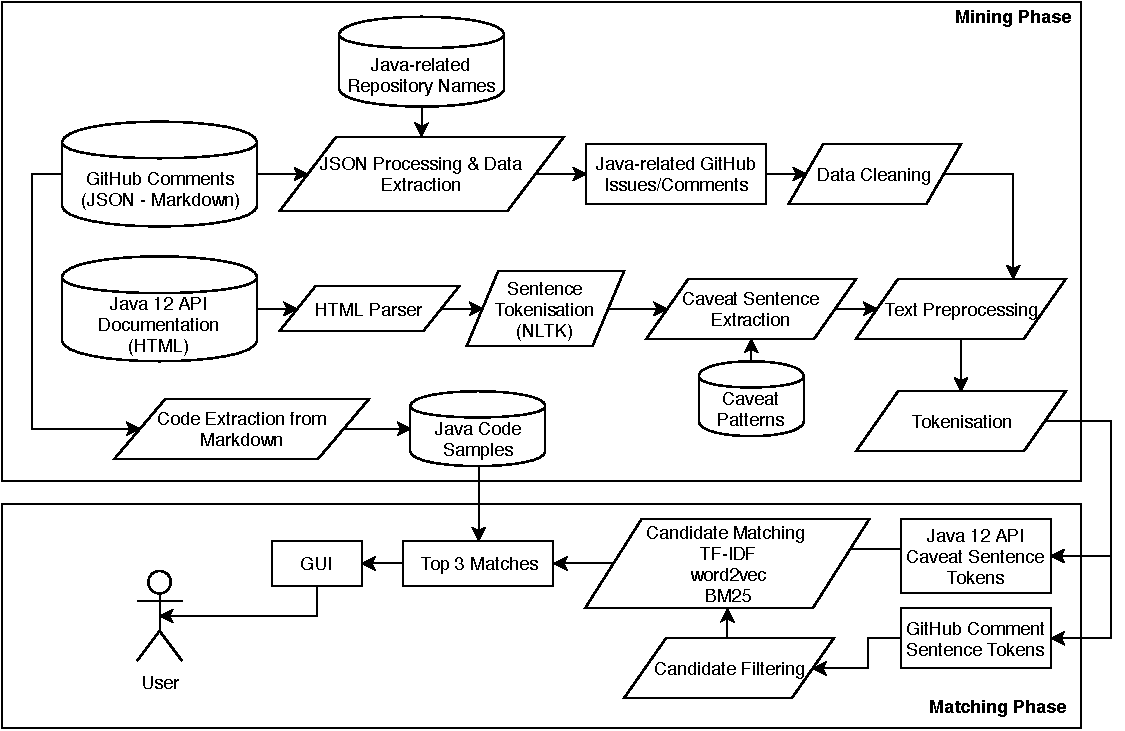
\includegraphics[width=\textwidth]{figs/github-architecture.pdf}
	\caption{Architecture design of the work for this chapter.}
\end{figure}
\flushleft

\subsection{TF-IDF Sentence Matching}
\label{subsec:info-tfidf}
TF-IDF is short for \textit{term frequency-inverse document frequency}. TF is based on the frequency of a term within a document while IDF refers to the inverse of the number of documents that contain the given term \cite{robertson2004understanding}. TF-IDF is computed as $TF\cdot IDF$, which is the multiplication of two measures. The formal definition of IDF is shown in Equation \ref{idf}, where $t$ is a token and $D$ is the documents in the corpus (a collection of documents). The overall motivation for TF is based on the assumption that meaningful words tend to appear more often within a document. However, this assumption means common terms such as ``the'' and ``a'' would be incorrectly emphasised. The IDF is therefore used to minimise the weights of words that appear frequently across the entire corpus. \\
The TF-IDF heuristic is a widely used technique for information retrieval systems that have been successful in several cases \cite{tfidf-explain}. For sentences, TF-IDF typically follows a bag-of-words approach in which vectors have a length equal to the vocabulary size and each component of the vector corresponds to the TF-IDF score of a single term.

\begin{equation}
\label{idf}
idf( t, D ) = log \frac{ \text{| } D \text{ |} }{ 1 + \text{| } \{ d \in D : t \in d \} \text{ |} }
\end{equation}

\subsection{Word2Vec Embedding}
\label{subsec:info-w2v}
Word2vec involves a computationally efficient neural network that is trained to learn and produce word embeddings. The original motivation for this was to capture contextual information such that words could be predicted in a sequence of words \cite{mikolov2013efficient}. The two models that can be used with word2vec is Continuous Bag-of-Words (CBOW) and Skip-Gram, though only an overview of Skip-Gram will be provided as it is the model used for sentence embedding in this chapter. The Skip-Gram model effectively predicts surrounding words given the current word and has the property that ``simple vector addition can produce meaningful results'' \cite{mikolov2013distributed}. An example of this provided in \cite{mikolov2013distributed}. Suppose \textit{vec(x)} represents the vector form of word $x$, then vec(``Germany'') + vec(``capital'') would result in a vector close to vec(``Berlin''). A simple method for applying word embeddings to sentence embeddings is to use the sum of the word vectors of a sentence. This is the method used for sentence embeddings in \ref{subsec:info-candidate-match}.

\subsection{BM25 Ranking}
\label{subsec:info-bm25}
BM25 is a ranking function that outputs the relevance of a document relative to other documents for a some query. It is based on a probabilistic model and is computed from Equation \ref{eq:bm25}, where $f(q_i, D)$ is the term frequency of term $q_i$ (the $i^{th}$ term in document $D$), $|D|$ is the document length, $k_1$ and $b$ are tuning variables, and $IDF'$ is an alternative version of IDF that is defined by Equation \ref{eq:bm25-idf} \cite{Manning:2008:IIR:1394399}. In particular, $b=0.75$ and $k_1 \in [1.2,2]$ are reasonable values reported by \citeauthor{Manning:2008:IIR:1394399}. The values $b=0.75$ and $k_1$ were therefore used in \ref{subsec:info-candidate-match}. BM25 was considered a state-of-the-art model for information retrieval in previous years \cite{perez2009integrating}. It is noted that since the BM25 scores are only comparable for a specific query, they can be normalised to the range 0-1 with 0 representing the least amount of relevance and 1 representing the highest. This allows its ranking score to be used in conjuction with cosine similarity for sentence matching.

\begin{equation} \label{eq:bm25} 
\text{score}(D,Q) = \sum_{i=1}^{n} \text{IDF'}(q_i) \cdot \frac{f(q_i, D) \cdot (k_1 + 1)}{f(q_i, D) + k_1 \cdot (1 - b + b \cdot \frac{|D|}{\text{avgdl}})} 
\end{equation}

\begin{equation} \label{eq:bm25-idf} 
\text{IDF'}(q_i) = \log{\frac{N - n(q_i) + 0.5}{n(q_i) + 0.5}}
\end{equation}

\section{Implementation}
\label{sec:info-implement}
Implementation of the data retrieval and extraction of GitHub comments alongside Java 12 API caveats was completed in Python 3.6. In particular, the Gensim library was used to apply word2vec sentence embedding to GitHub comment sentences and Java API caveat sentences. The Sci-kit library was used to obtain sentence vectors from TF-IDF sentence embedding. Rankings for BM25 were computed manually using its associated function. Section \ref{subsec:info-github-extract} describes the collection of GitHub data and its extraction for sentence embedding and matching. Section \ref{subsec:info-caveat-extract} provides an overview of the Java 12 API documentation and extraction of its API caveat sentences. Section \ref{subsec:info-data-preprocess} explains the sentence preprocessing steps performed, followed by filtering steps to ease the scope of sentence matching required for the large sets of sentences (Section \ref{subsec:info-candidate-filtering}). Section \ref{subsec:info-sentence-embedding} illustrates the tools used for sentence embedding, and finally, Section \ref{subsec:info-candidate-match} describes how the Java 12 API caveat sentences were matched with sentences from GitHub comments.

\subsection{GitHub Data Extraction}
\label{subsec:info-github-extract}
There are three notable sources for GitHub data: (1) the GitHub Representational State Transfer (REST) API, (2) the GitHub Archive project, and (3) GitHub itself by cloning a repository. For this project, the GitHub REST API and GitHub Archive project was utilised due to the memory and processing requirements of cloning each repository of interest with option 3. However, the GitHub REST API contains several limitations that inhibit its usefulness for a large corpus of community text. This includes limitations on the request rate (30 requests per minute using the ``search'' API) and query options (e.g. it does not allow complex searches such as ``all GitHub issues associated with Java projects in January'', or more than 100 results per query). For option 2, GitHub Archive is a project that creates hourly archives of all GitHub data starting from 2/12/2011 as JSON objects. The archives include over 20 event types that are provided by GitHub such as the creation of an issue or comment. For issues and comments, the raw text of the posts is included in Markdown format, which represents the community text of interest.  However, these objects do not provide metadata for which programming languages or APIs are relevant. This makes it difficult to filter out irrelevant posts for information retrieval systems in later steps.
Thus, we combine the queries of the GitHub REST API to identify the repositories that are Java related, then link them with the community text captured by GitHub Archive.\bigbreak

In more detail, GitHub provides a REST API to allow developers to query for data on GitHub such as metadata about a particular repository or the number of repositories use some programming language. The REST API imposes a rate limit on user requests to prevent flooding of the GitHub servers. For this API, its  ``search'' functionality is the main solution for searching repositories or issues given specific conditions such as the time in which it was created. The API does not provide functionality to search for the contents of GitHub issues and comments across multiple repositories. Furthermore, the API is limited to a maximum of 100 results for a single query. The API is therefore only useful for finding which repositories contain Java code. The rate limit imposed is circumvented by performing numerous HTTP GET requests in sequence. This involves sending queries with a timer between each request and modified query parameters for (daily) creation times. A time window of 2009 to 2019 was chosen alongside a restriction of at least 2 ``stars'' to reduce the scope of projects collected to those that contained Java code and likely had more than 1 developer involved (as the number of stars a repository contains can be used to gauge its popularity). The PyGitHub Python library, in particular, is used to implement these queries to the GitHub REST API. Overall, collecting repository names of Java-related projects from 2009-2019 projects that contain at least 2 stars yields 291,152 results. \bigbreak

GitHub Archive captures an event known as ``IssueCommentEvent'', which contains various information about a comment for a particular issue. The archives are saved hourly. Therefore, a script is used to automate the process of downloading all archived data for 2018. Note that only data from 2018 is collected to reduce the amount of time required for querying the entire dataset and as an initial study. Multiprocessing is used in particular with a Python script to perform concurrent downloads and reduce the time required for data collection. After this, the extraction of relevant ``IssueCommentEvent'' objects is performed by checking whether the associated repository of a comment is Java related based on the list attained from the GitHub REST API. Notable information of these objects such as the text body of an issue comment and its title is extracted for natural language processing in later steps. Overall, this extraction process results in 627,450 GitHub issues and 1,855,870 issue comments to be collected.

\subsection{Java 12 Documentation Caveat Extraction}
\label{subsec:info-caveat-extract}
To begin extracting API caveats, the API documentation must first be collected. At the time of writing, the Java Standard Edition 12 API was chosen for analysis, which was the latest Java version and documentation available. This API was chosen as it comprises the standard library for Java and is, therefore, expected to be the most generalised API used by most Java projects. Its documentation consists of Hypertext Markdown Language (HTML) pages for each class of the Java Development Kit (JDK) 12. In particular, the API documentation contains a webpage in HTML that lists the complete class hierarchy tree of the Java standard library.\footnote{https://docs.oracle.com/en/java/javase/12/docs/api/overview-tree.html} This information allows us to data crawl the entire Java API documentation. First, the Uniform Resource Locator (URL) of all classes are mined from the class hierarchy page by collecting all hyperlink references on the page found within the appropriate HTML \lstinline{section} element. The Beautiful Soup\footnote{https://pypi.org/project/beautifulsoup4/} library is used to parse the HTML content. The relative URLs of each class are found by locating list item elements (\lstinline{li}) then anchor elements (\lstinline{a}) residing within. From this, absolute URLs are constructed for 4,865 classes. Next, the HTML pages for each class is downloaded by recursively sending HyperText Transfer Protocol (HTTP) GET requests for each of the URLs generated. A total of 4,712 classes are found alongside 4,172 constructors and 33,827 methods. At this point, an important note to make for the Java SE 12 documentation is that it is automatically generated from comments in the source code implementation with the JavaDoc tool and is well-structured. For example, the parameters and possible exceptions for a method are consistently placed within certain HTML elements across all HTML pages. Hence, it is relatively simple to identify and extract sentences for each API element alongside additional information such as whether a method is deprecated from the existence of a \lstinline{div} element with the ``deprecationBlock'' Cascading Style Sheets (CSS) class for example.\bigbreak

The extraction of caveat sentences is performed by creating a set of regular expressions based on keywords and patterns identified in \cite{caveat-knowledge-graph}. These regular expressions allow us to check whether arbitrary strings contain some predefined patterns. API caveat sentences are then identified by checking if one of the regular expressions finds a match within a sentence from the API. This is executed recursively for all of the HTML pages, in which 107,601 caveat sentences are found. Of these sentences, 9,964 are regarded as \textit{class level sentences}, which are sentences that describe the overall class and are located in the class description section of API documents (typically at the top of each API document). A snippet of this is shown in Figure \ref{fig:class-sents}. The Java 12 API is also structured such that each method/field/constructor for a given class contains a self-contained section that describes details specific to that element. An example of this is shown in Figure \ref{fig:api-doc-eg}. We refer to the sentences that appear in the description of these sections as \text{element level sentences}. A total of 37,578 element level sentences are identified as caveat sentences. Other notable locations for sentences are sections that describe the parameters, exceptions or return value (if it is a method) of a particular API element. We refer to sentences found in those areas as \textit{parameter sentences}, \text{exception sentences} and \textit{return sentences} respectively. The number of caveat sentences found at these levels is 12,614, 32,623 and 11,765. Besides this, it is discovered that 1,522 API elements of the Java 12 API are deprecated. \\

\begin{figure}[h]
	\label{fig:class-sents}
	\centering
	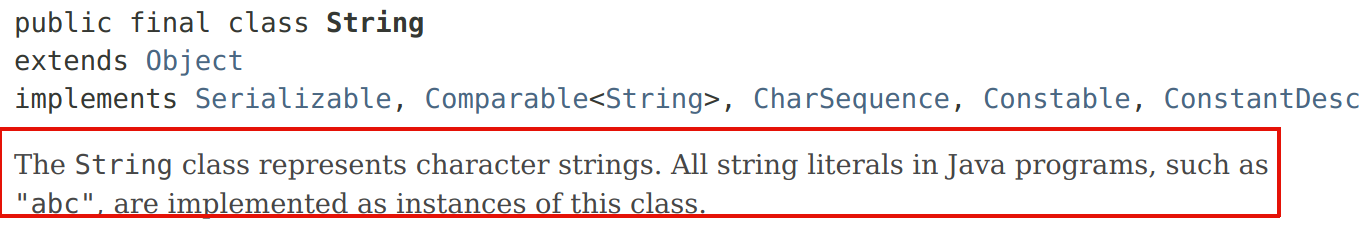
\includegraphics[width=\textwidth]{figs/class-sents-highlight.png}
	\caption{Example of the description section for the Java \lstinline{String} API documentation. Sentences located in this area (highlighted in red) are referred to as \textit{class level sentences}.}
\end{figure}

\begin{figure}[h]
	\label{fig:api-doc-eg}
	\centering
	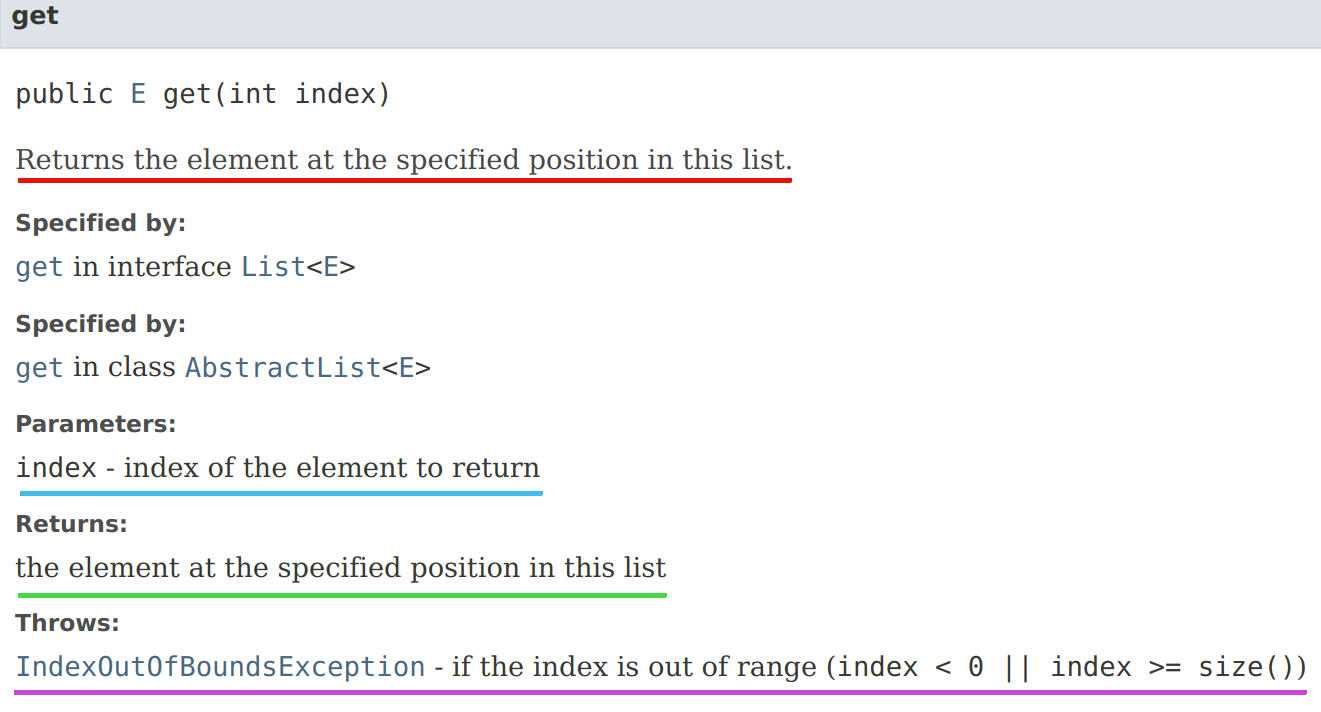
\includegraphics[width=\textwidth]{figs/api-doc-eg-highlight.png}
	\caption{Example of the API documentation for \lstinline{ArrayList.get(int index)}. Sentences located in the red underlined section, blue underlined section, green underlined section, and purple underlined section are referred to as \textit{element sentences}, \textit{parameter sentences}, \textit{return sentences} and \textit{exception sentences} respectively.}
\end{figure}
\clearpage

\begin{table}[h]
	\centering
	\begin{tabular}{@{}lll@{}}
		\toprule
		\textbf{Category} & \textbf{Subcategory} & \textbf{Syntactic Pattern Examples} \\ \midrule
		\multirow{5}{*}{Explicit} & Error/Exception & \begin{tabular}[c]{@{}l@{}}``insecure'', ``susceptible'', ``error'',\\ ``null'', ``exception'', ``susceptible'',\\ ``unavailable'', ``not thread safe'',\\ ``illegal'', ``inappropriate'',\end{tabular} \\ \cmidrule(l){2-3} 
		& \multicolumn{1}{l}{Recommendation} & \multicolumn{1}{l}{\begin{tabular}[c]{@{}l@{}}``deprecate'', ``better/best to'',\\ ``recommended'', ``less desirable''\\ ``discourage''\end{tabular}} \\ \cmidrule(l){2-3} 
		& Alternative & ``instead of'',``rather than'',``otherwise'' \\\cmidrule(l){2-3} 
		& Imperative & ``do not'' \\\cmidrule(l){2-3} 
		& Note & ``note that'', ``notably'', ``caution'' \\\hline
		\multirow{2}{*}{Restricted} & Conditional & \begin{tabular}[c]{@{}l@{}}``under the condition'', ``whether ...'',\\ ``if ...'', ``when ...'', ``assume that ...''\end{tabular} \\\cmidrule(l){2-3}
		& Temporal & ``before'', ``after'' \\\hline
		\multirow{3}{*}{Generic} & Affirmative & \begin{tabular}[c]{@{}l@{}}``must'', ``should'', ``have to'',\\ ``need to''\end{tabular} \\
		& Negative & ``do/be not ...'', ``never'' \\
		& Emphasis & ``none'', ``only'', ``always'' \\ \hline 
	\end{tabular}
	\caption{API caveat categories and syntactic patterns from \cite{caveat-knowledge-graph}.}
	\label{tab:caveat-keywords}
\end{table}

\subsection{Data Preprocessing}
\label{subsec:info-data-preprocess}
Data cleaning and text preprocessing are required to allow NLP techniques/models to perform correctly. Numerous preprocessing steps are therefore applied to prepare the sentences for word and sentence embedding. In particular, the comments are in Markdown format, allowing simple removal of unwanted elements such as code blocks (which are wrapped between a pair of \lstinline{```}). Furthermore, all URLs, supplementary white space characters, apostrophes and punctuation (except for full stops appearing after a word) are removed. In particular, full stops are retained in consideration of inline code such as ``array.length''. The removed parts of the text are substituted with a white-space character so that individual components of references to API elements (e.g. ``array.length'') can be separated correctly during word tokenisation.  For sentence tokenisation, which separates a paragraph into its sentences, full stops that were followed by a space were used to identify the split points.  We note that a custom sentence tokeniser is required to prevent cases where full stops within inline code would result in a sentence split. Finally, word tokenisation is performed for each preprocessed sentence. This simply involves splitting the sentences based on white space characters such that each sentence is represented as a list of tokens. This representation is essential for further NLP tasks as it simplifies parsing/processing for computers. \bigbreak

Next is the removal of a customised set of English stop words provided by the NLTK library\footnote{https://www.nltk.org/index.html}. Stop words are common words that add little value/meaning for NLP such as ``a'' and ``is''. For the GitHub data, stop words that were of length 1 were retained such that single character variable names like ``i'' (commonly used by Java programmers in \lstinline{for} loops) are retained. Overall, preprocessing and tokenisation of all GitHub comments results in 1,855,870 tokenised sentences. It is noted here that in \cite{jiamou}, two additional steps are performed for the sentences: (1) coreference resolution, where pronouns such as ``it'' and ``this'' is substituted with the closest API names, and (2) lexicon construction in which an API lexicon (i.e. a vocabulary set of API element names) is constructed from the code of question and answer posts of Stack Overflow. Both of these steps are intended to reduce the complexity and noise of sentence embedding and matching. However, an initial search of the GitHub data via Google found that finding examples of API misuse from GitHub data is significantly more difficult than with Stack Overflow. For simplicity, step 1 is therefore ignored. Step 2 is reduced to keyword matching of both the API element name and its associated class name in Section \ref{subsec:info-candidate-filtering} when determining the relevant API elements of each GitHub comment, and hence, the list of potentially relevant API caveats for those comments.

\subsection{Candidate Filtering}
\label{subsec:info-candidate-filtering}
The caveat sentences that were associated with deprecated API elements or were not an element sentence, parameter sentence or exception sentence were filtered. In particular, the sentences for deprecated elements are ignored because those caveats are typically obvious to developers as Integrated Development Environments (IDEs), software that support programmers with development, highlight cases where an API element is deprecated. This is accomplished using the \lstinline{@Deprecated} annotation for Java that is tagged onto deprecated methods by API developers. I only focus on element, parameter and exception sentences to reduce the scope of sentences during sentence matching with GitHub comments and because these sentences were found to describe the most explicit caveats (such as  the ``index < 0 || index >= size()'' constraint in the exception sentence of Figure \ref{fig:api-doc-eg}). It is hypothesised that these explicit types of caveats are the most likely caveats to be matched to community sentences as they would require some form of paraphrasing to explain and would result in obvious errors and exceptions to be thrown.\bigbreak

For reference, it is observed that several caveat sentences extracted are invalid: they contain snippets of code or do not necessarily specify a constraint for users. Example of caveat sentences containing code snippets is shown in Listing \ref{invalid-caveat-1}, \ref{invalid-caveat-2} and \ref{invalid-caveat-3}. An example of an API caveat that does not specify a constraint is the class level sentence ``Java implementations must use all the algorithms shown here for the class Random, for the sake of absolute portability of Java code.'' from the \lstinline{Random} class\footnote{https://docs.oracle.com/en/java/javase/12/docs/api/java.base/java/util/Random.html}. To counteract sentences containing code snippets, those that exceeded an arbitrarily (generous) limit of 400 characters were excluded from further analysis and sentence matching. The other type of invalid caveat sentences were ignored as they appeared to represent a small portion of the extracted caveats.
In addition to this, it was noted that matching all of the GitHub issue comment sentences against every API caveat sentence would require significant processing time/power. The potentially relevant API caveats for each GitHub comment were therefore identified first to filter out non-relevant API caveats. This was achieved by concatenating the text of each comment and their associated GitHub issue, transforming the string to lowercase characters only, and performing a sub-string search for the (lowercase) class name and API element name of the API caveats. Caveats that were potentially relevant to more than 1000 GitHub comments were restricted to those 1000 GitHub comments to further reduce computation. This restriction involved 213 of the 21,932 API elements from the Java 12 documentation. We note that this limits the search area of sentence matching for those API caveats considerably, but is acceptable for an initial attempt of sentence matching. The total number of caveat sentences after preprocessing and all filtering functions totalled 73,831.\bigbreak

For GitHub comments, those that were not attached to an issue containing a code block were filtered. This is because the overall purpose of sentence matching is to indirectly link API caveats to code examples. From the dataset, 85,318 issues contained a code block with  290,019 associated comments. Those comments contained 629,933 sentences in total. The next step for sentence matching was to perform sentence embedding.

\clearpage
\begin{lstlisting}[label=invalid-caveat-1,caption={An example of a caveat sentence extracted from the \lstinline{javax.swing.Spring} documentation containing some snippets of code or mathematical expressions},float,frame=tb,numbers=none,language=None,linebackgroundcolor={\lstcolorlines{4,5,6}}]
If we denote Springs as [a, b, c], where a <= b <= c, 
we can define the same arithmetic operators on Springs:

[a1, b1, c1] + [a2, b2, c2] = [a1 + a2, b1 + b2, c1 + c2]
-[a, b, c] = [-c, -b, -a]
max([a1, b1, c1], [a2, b2, c2]) = [max(a1, a2), max(b1, b2), max(c1, c2)]
\end{lstlisting}

\begin{lstlisting}[label=invalid-caveat-2,caption={An example of a caveat sentence extracted from the \lstinline{java.security.cert.X509CRL} documentation explaining the structure of a \lstinline{TBSCertList} object.},float,frame=tb,numbers=none,language=None,linebackgroundcolor={\lstcolorlines{3,4,5,6,7,8,9,10,11,12,13,14,15,16,17}}]
The ASN.1 definition of tbsCertList is:

TBSCertList  ::=  SEQUENCE  {
	version                 Version OPTIONAL,
	-- if present, must be v2
	signature               AlgorithmIdentifier,
	issuer                  Name,
	thisUpdate              ChoiceOfTime,
	nextUpdate              ChoiceOfTime OPTIONAL,
	revokedCertificates     SEQUENCE OF SEQUENCE  {
	userCertificate         CertificateSerialNumber,
	revocationDate          ChoiceOfTime,
	crlEntryExtensions      Extensions OPTIONAL
	-- if present, must be v2
	}  OPTIONAL,
	crlExtensions           [0]  EXPLICIT Extensions OPTIONAL
	-- if present, must be v2
}
\end{lstlisting}

\clearpage

\begin{lstlisting}[label=invalid-caveat-3,caption={An example of a caveat sentence extracted from the \lstinline{java.text.BreakIterator} documentation that contains some sample code.},float,frame=tb,numbers=none,language=None,linebackgroundcolor={\lstcolorlines{3,4,5,6,7,8,9,10,11,12,13,14,15,16,17}}]
Creating and using text boundaries:

public static void main(String args[]) {
	if (args.length == 1) {
		String stringToExamine = args[0];
		//print each word in order
		BreakIterator boundary = BreakIterator.getWordInstance();
		boundary.setText(stringToExamine);
		printEachForward(boundary, stringToExamine);
		//print each sentence in reverse order
		boundary = BreakIterator.getSentenceInstance(Locale.US);
		boundary.setText(stringToExamine);
		printEachBackward(boundary, stringToExamine);
		printFirst(boundary, stringToExamine);
		printLast(boundary, stringToExamine);
	}
}
\end{lstlisting}

\subsection{Sentence Embedding}
\label{subsec:info-sentence-embedding}
Sentence embedding provides a method of comparing the similarity of two sentences by mapping them to vectors and computing the angle between the two vectors. The process of representing variable-length sentences as fixed-length vectors has been a major research topic related to deep learning approaches for NLP \cite{adi2016fine}.
TF-IDF based vector representations were created for the sentences using the Scikit-learn library\footnote{https://scikit-learn.org/}. This involved the class \lstinline{TfidfVectorizer} and calling its \lstinline{fit_transform} function to create vectors for all API caveat sentences. For word2vec sentence embedding, the \lstinline{word2vec} class from the \lstinline{gensim} library is imported and used. Note that the input for sentence embedding is the preprocessed, tokenised and filtered forms of caveat sentences and Github comment sentences. Hence, TF-IDF and word2vec vectors were generated for the 629,933 Github comment sentences and 73,831 caveat sentences.

\subsection{Candidate Matching}
\label{subsec:info-candidate-match}
Sentence matching is accomplished using cosine similarity for the sentence embedding vectors. For BM25, its function already outputs a ranking score for a particular match pair and does not require further computations. To evaluate the cosine similarity of the vectors, each of the 73,831 caveat sentence vectors is compared to a unique subset of the 629,933 sentence vectors from GitHub comments that are deemed potentially relevant (this was computed in Section \ref{subsec:info-candidate-filtering}). The equation in \ref{cosine} is then used to compute the similarity scores. A similarity score of 1 represents high sentence similarity between two sentence vectors, while 0 represents dissimilarity. Given that BM25 ranks the sentence vectors relevant to each other, the BM25 scores were then normalised to the range 0 and 1, with 1 being representing the highest similarity. Thus, scores ranging from 0-1 were computed for each caveat sentence against their subset of potentially relevant GitHub comment sentences for TF-IDF, word2vec, and BM25. A weighted combination of BM25 and word2vec was then considered (with equal weightings for both scores) since using both approaches could be expected to balance the advantages/disadvantages of sentence embeddings and a probabilistic model. \\

\begin{equation}
\label{cosine}
\cos ({\bf A},{\bf B})= {{\bf A} {\bf B} \over \|{\bf A}\| \|{\bf B}\|} = \frac{ \sum_{i=1}^{n}{{\bf A}_i{\bf B}_i} }{ \sqrt{\sum_{i=1}^{n}{({\bf A}_i)^2}} \sqrt{\sum_{i=1}^{n}{({\bf B}_i)^2}} }
\end{equation}

To evaluate the performance of each information retrieval system (and the approach in general), a statistical sampling size from a statistical sampling method from \cite{singh2013elements} is used. Specifically, the minimum number of samples required to ensure the estimated population mean is within a given confidence level and error margin can be calculated by the formula:

\begin{equation}
\label{sample}
min=\frac{\frac{z^2\times 0.25}{e^2}}{1 + \frac{(\frac{z^2\times 0.25}{e^2} - 1)}{p}}
\end{equation}

Where $z$ is the z-score associated with the desired confidence level, $e$ is the error margin and $p$ is the population size.
From this, an estimated sampling size of 383 is required given a 95\% confidence interval, 5\% error margin and population size of 73,831 (i.e. the number of preprocessed and filtered caveat sentences). However, a population size of 384 was used for consistency with \cite{xiaoxue} in which notably more API caveat sentences from the Android documentation were analysed (160,112). The precision at K metric (precision@k) is chosen for a simplistic, initial evaluation of a query for the information retrieval systems, where K is set to 3 to reduce the amount of manual labelling required for all approaches (TF-IDF, word2vec, BM25 and word2vec + BM25). This is then combined with the mean average precision metric to quantify the overall performance of the systems across multiple queries. Hence, I generate a different random sample of caveat sentences for each information retrieval system and collect the top 3 results of those queries. Note that separate sampling is performed for each model since we also aim to observe and evaluate the variety of caveat sentences and their relevant GitHub comments for an initial study. The random sampling resulted in 959, 936, 1129 and 1051 results for the TF-IDF, word2vec, BM25, and word2vec + BM25 information retrieval systems for manual labelling. The sampling sizes are inconsistent because some caveats sentences can have less than 3 GitHub comments that are deemed potentially relevant in the given dataset.



\section{Results}
\label{sec:info-results}
Labelling of the sentence matching results was conducted by manually checking whether the given API caveat appeared to be relevant to the GitHub comment containing the matched sentence. In particular, the caveat is compared against the entire GitHub comment such that contextual information from the GitHub comments can also be considered. Each query and result pair were annotated with either \textit{relevant} or \textit{non-relevant} based on whether the GitHub comment referred to the API caveat. A significantly small percentage of the results were found to be relevant to their API caveat query, with only 9, 16, 5 and 11 results identified as relevant for the TF-IDF, word2vec, BM25, and word2vec + BM25 information retrieval systems. In other words, only about 1\% of the query results for the random samples are relevant to their API caveats. The mean average precision@3 for all of the information retrieval systems is approximately 0. It is noted that using a similar version of the code on another work\footnote{\url{https://xin-xia.github.io/publication/ase192.pdf}} based on Stack Overflow and Android API caveats showed promising results. I, therefore, perform an analysis of these findings to understand why the systems performed poorly for GitHub data.\\

\clearpage

\begin{lstlisting}[label=error-log,caption={Example of a GitHub comment containing an error log from \url{https://github.com/ChrisRM/material-theme-jetbrains/issues/863}},float,frame=tb,numbers=none,language=None]
similar problem just now, Linux (CentOS), upgrading from 2018.1 to 2018.2. 
(I use the Darcula theme, and this stack trace is suggestive...)\r\n\r\njava.lang.ClassCastException: java.lang.Boolean cannot be cast to com.intellij.openapi.actionSystem.ex.ComboBoxAction\r\n\tat com.intellij.ide.ui.laf.darcula.ui.DarculaButtonUI.
getComboAction(DarculaButtonUI.java:75)\r\n\tat com.intellij.ide.ui.laf.darcula.ui.DarculaButtonUI.
getDarculaButtonSize(DarculaButtonUI.java:236)\r\n\tat com.intellij.ide.ui.laf.darcula.ui.DarculaButtonUI.
...
\end{lstlisting}

To verify the results, the API caveat queries of the random samples and the results returned by the information systems are examined. It was found that numerous GitHub comments contained code or error logs as text. Manually checking the preprocessing/filtering steps on these comments, I found that several sentences were not preprocessed/filtered correctly because of missing code tags in the Markdown text. In other words, users occasionally include code or error logs besides natural language text. An example of this is shown in \ref{error-log}, where the error logs are inline with actual sentences. Note that the example has been truncated and long lines were split for better viewing. This would result in the text from those code and error logs to be processed as natural language words during information retrievals. This is a particularly hard problem to fix given that code and error logs do use a single, specific template and how they are presented is dependent on the user. Besides this, it was noted that the repositories associated with GitHub comments could utilise many different APIs. This means that the text from GitHub comments could be related to numerous APIs and their caveats, which is not typically distinguished. \bigbreak

In comparison to Stack Overflow, users on Q\&A platforms can usually ``tag'' their questions under a certain topic (such as Android or a specific API). However, GitHub does not provide that functionality as its community text options are intended for bug reports or suggestions. This means it is much harder to differentiate the GitHub comments by API relevance. The consequence of this was seen in cases where the correct API class name and element name of a given API caveat was mentioned in the GitHub comment, but were generic names (e.g. \lstinline{truncate}, \lstinline{compareTo}, \lstinline{getOffset}), that were associated with a different API. It is noted that perhaps linking caveats for a more specific API (such as specific Java libraries like ReactiveX\footnote{http://reactivex.io/} or OkHttp\footnote{https://square.github.io/okhttp/}) could yield better results for GitHub data since those projects have their own GitHub repositories. Issues and comments for those repositories would therefore likely be related to their respective APIs. Another possible reason for the negative results is the caveat sentences from the Java API. It was observed that some of the caveats could be considered too generic. For example, the \lstinline{set} and \lstinline{get} methods of the \lstinline{java.util.ArrayList<E>} class both share the same sentence: ``IndexOutOfBoundsException - if the index is out of range (index < 0 || index >= size())''. Even with the process of coreference resolution used in \cite{jiamou} to deal with similar caveat sentences, it is difficult to distinguish which API element the caveat relates to.
An example where unrelated classes and methods of the Java API contain similar caveat sentences is from the constructor of \lstinline{java.util.HashMap<K,V>} that says ``NullPointerException - if the specified map is null'' and from the \lstinline{addAll} method of \lstinline{java.util.ArrayList<E>} that says ``NullPointerException - if the specified collection is null''. \bigbreak

Another possible reason that GitHub is considerably worse for linking API caveat sentences is that its community text serves a different purpose compared to Q\&A websites such as Stack Overflow. In particular, community text regarding API caveats would likely be in the format of a bug report, and answers to specific caveats can already be found on platforms catered to answering those caveats (i.e. Stack Overflow). Other forms of natural language that could be analysed for API caveat linkage is \textit{commit} messages. Commits are typically individual file changes, where developers can attach a short message provide an overview of what changes were made. Another option is with \text{pull requests}, which contains a set of changes and longer discussions and reviews of these changes. However, both commits and pull requests are non-viable approaches for linkage as it is difficult to identify which code examples are associated with their natural language text. This is because both options can involve changes made to different lines of code files, and their descriptions for the changes made must be similar to the descriptions of API caveats. Code that has been uploaded to GitHub has also (likely) been executed, meaning explicit types of API caveats that result in exceptions/errors would be fixed beforehand.\bigbreak

Ultimately, it can be seen that due to the usage of same/similar sentences for different API elements, the inclusion of many different APIs on GitHub, and different purpose of GitHub results in a significant lexical gap for the Java 12 API caveat sentences and community text from GitHub. Though, a closer look at the caveat sentences and information retrieval results, in general, allowed an important observation to be made: caveats from exception sentences tend to describe explicit constraints in the Java 12 API documentation. These types of caveats would, therefore, be more applicable in a real-time setting where code could be analysed before it was released to GitHub. It is noted that these exception level caveats represent a large proportion of the API caveats (32,623 of 107,601 sentences).   Finding a method to apply these constraints directly to code would be more beneficial in terms of both preventing issues with API caveats and helping programmers understand them. Overall, the poor results from this approach lead to the alternative idea of representing exception level caveats in a way where code analysis could be performed in Chapter \ref{cha:codeAnalysis}.

\section{Summary}
\label{sec:info-summary}
This chapter described the background work that is used for linking API caveats to code examples and focuses on extending the solutions to a different domain: GitHub. The data of GitHub is of interest for API caveat linkage because it is another community platform that contains an abundance of code. However, GitHub is inherently different from the focus of \cite{jiamou} and \cite{xiaoxue}, which was strictly Q\&A community websites. The Java 12 API documentation was used instead of the Android API documentation for API caveats as it could be generalised to more projects on GitHub. After extraction, 107,601
caveat sentences are found for the Java 12 API. For GitHub data, the GitHub Archive project is used to collect all GitHub events throughout 2018. The complete list of Java-related projects that had at least 2 stars is collected using the GitHub REST API, finding 291,152 projects. A total of 1,855,870 GitHub comments related to Java in 2018 are then identified from the GitHub Archive dataset. The sentences underwent data preprocessing, filtering, and sentence embedding (based on TF-IDF and word2vec) to perform sentence similarity computations between the two GitHub comment sentences and Java 12 API caveat sentences. After filtering, this involved matching 73,831 caveat sentences against 629,933 sentences from GitHub comments. \bigbreak

Information retrieval systems were created based on TF-IDF, word2vec, BM25, and word2vec + BM25, with caveat sentences used as queries and query results being GitHub comment sentences (ranked according to their relevance). Manual labelling was performed to measure the performance of the information retrieval systems. A statistical random sampling method was used with a 95\% confidence interval and 5\% error margin. It was found that 1\% or less of the query results were found relevant for all of the information systems used. The cause of this was discussed and suspected as a result of the differences in GitHub as a community platform in comparison to Q\&A websites. GitHub data is also polluted with many different APIs that makes it harder to discern which API arbitrary text is associated to.\\
In Chapter \ref{cha:codeAnalysis}, I take a more direct approach to linking API caveats to code by transforming API caveat sentences into \textit{caveat contracts} and conducting static code analysis.

\chapter{API Contracts Construction with Static Code Analysis}
\label{cha:codeAnalysis}
This chapter explains the concept of constructing caveat contracts from API caveats. In particular, it provides an overview of how caveat sentences from the Java 12 API documentation can be used to construct coding rules similar to code contracts. Applications of static code analysis for these caveat contracts are then explored, with one sample implementation for detecting bugs in real-time described.\\

\noindent
Section \ref{sec:contract-intro} provides background information for code contracts and an overview of the work conducted for this Chapter: constructing code contracts from API caveat sentences and using static code analysis to apply the contracts to code in real-time. \\

\noindent
Section \ref{sec:contract-design} describes the design framework for generating and using code contracts. This includes a statistical analysis on the Java 12 API caveats, a description of the idea used for extracting information from caveat sentences for code contracts construction, and the concept of checker programs that can utilise the code contracts. \\

\noindent
Section \ref{sec:contract-implement} explains the implementation of API contracts construction and static code analysis in an IntelliJ proof-of-concept plugin. \\

\noindent
Section \ref{sec:contract-results} showcases the IntelliJ plugin developed that uses caveat contracts to detect API misuse. \fix{Extensions of this concept are also addressed.}

\section{Introduction}
\label{sec:contract-intro}
Code contracts are a concept derived from object-oriented principles in which preconditions, postconditions, and invariants are defined for different software components. Specifically, the principle of ``design by contract'' suggests the use of specifications for code referred to as contracts. This improves code correctness and robustness as software components can only interact via obligations to code contracts. Using this concept, we can reduce the problem of linking API caveats to source code to the problem of mapping API caveats to code contracts, which we refer to as \textit{API caveat contracts} or simply \textit{caveat contracts} in this thesis. This can be used in real-time to provide feedback during the programming/development process in regards to API caveats. As a continuation of the previous chapter, I perform a statistical analysis of several caveat types for the Java 12 API documentation based on the work by \cite{zhou-directive}. I then propose a parsing technique to construct contracts from API caveats exception sentences, which represent a large proportion of API caveats for the Java 12 API and typically result in exceptions to be thrown. This extends upon the parsing techniques used by both \cite{zhou-directive} and \cite{blasi2018translating} to collect a subset of API caveats related to explicit constraints including range limitations or not-null constraints. From this, I construct a total of 4,694 unique caveat contracts. Finally, I develop a checker plugin for IntelliJ that can use the caveat contracts to highlight violations of these API contracts in real-time. \\

\section{Design}
\label{sec:contract-design}
The first step to generating contracts for API caveats is the extraction of API caveat sentences. This process is described in the previous chapter (Section \ref{subsec:info-caveat-extract}), and all caveat sentences extracted are re-used for this chapter. We recall that caveat extraction for the Java 12 reference documentation yields 
107,601 caveat sentences, where a significant proportion of the sentences are exception sentences or parameter sentences (approximately 30\% and 11\% respectively). These are analogous to the subset of constraints identified and focused in \cite{zhou-directive} and found to represent the largest portion (43.7\%) of API documentation in \cite{directives-study}. From \cite{zhou-directive}, a set of heuristic rules was created from manual inspection that classifies the types of these constraints as (1) nullness not allowed, (2) nullness allowed, (3) type restriction and (4) range limitation. In particular, sentence normalisation techniques were used in both \cite{zhou-directive} and \cite{blasi2018translating} in preparation for parsing techniques. The NLP techniques of POS tagging (identification of part-of-speech categories like nouns for words), dependency parsing (identification of the syntactic structure of sentences) and open information extraction (extraction of relation tuples from plain-text)
are then applied to construct FOL expressions representing the constraints. An SMT solver can then be used to compare whether two FOL expressions were equivalent. This was used in \cite{zhou-directive} by comparing API documentation constraints with the associated code implementations to check whether API documentation was defective. The FOL expressions constructed from code involved traversing the ASTs of programs to extract exceptions thrown and the conditions for those exceptions.\bigbreak

For this thesis, I mainly focus on the {not-null} and \textit{range limitation} constraints identified by \cite{zhou-directive} to reduce the scope of caveat mappings to contracts (given the diversity of API caveats). However, it should be noted that other categories of API caveats could also be transformed with other NLP techniques. Besides this, I base my parsing approach on the sentence normalisation technique used in the previously mentioned work. For static code analysis, I focus on the process used by \cite{zhou-directive} where relevant code elements are first identified, followed by an appropriate analysis of those elements. This can be used by a plugin for some IDE to highlight contract violations (API misuses) while coding. However, I note that another method used in \cite{code-examples}, which involves creating an alternative representation of code from ASTs containing only important features of an API method call, could also be used. Overall, the design architecture of the approach for this chapter is shown in Figure \ref{fig:contracct-architecture}.

\begin{figure}[h]
	\label{fig:contracct-architecture}
	\centering
	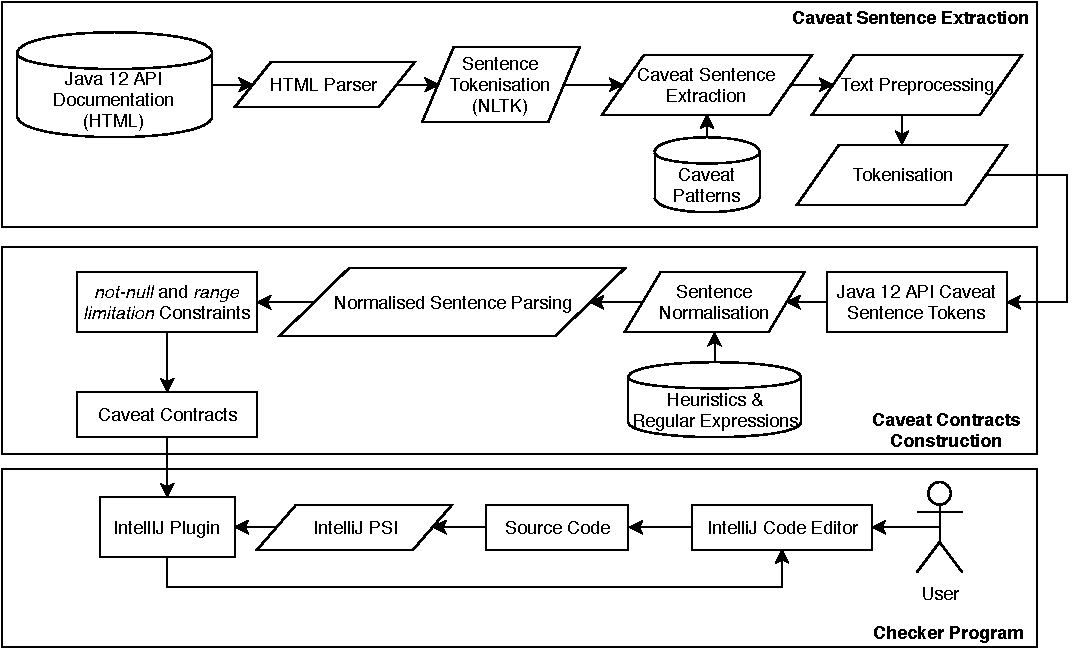
\includegraphics[width=0.8\textwidth]{figs/contract-architecture.pdf}
	\caption{Architecture design of the work for this chapter.}
\end{figure}

Section \ref{subsec:contract-caveat-statistics} provides an overview of the statistical analysis performed for the Java 12 API caveats. This is followed by Section \ref{subsec:contract-construct} that describes the design idea for parsing and extracting constraints from API caveats. Finally, Section \ref{sec:code-checker} gives an overview of ASTs and how checker programs can utilise caveat contracts.

\subsection{Java 12 Caveat Statistics Analysis}
\label{subsec:contract-caveat-statistics}
An observation on the exception sentences of the Java 12 documentation is their consistent structure. These sentences follow a template of ``\verb|exception - description|'', where \verb|exception| is the exception class thrown and \verb|description| describes conditions required for the exception to be thrown. An example of this is shown in Figure \ref{fig:api-doc-charAt}. It is noted that similar structures are used for other sentences such as the parameter sentences, which follow a template of ``\verb|param - description|'', where \verb|param| is the name of the parameter for a given method/constructor and \verb|description| is the actual sentence describing some information about \verb|param|.  Overall, this information can be used to trivially separate key parts of caveat sentences found within these sections (i.e. the subject and associated description). For parsing constraints, we are only interested in the description parts of exception sentences, as this is where constraints imposed are described. Therefore, only the descriptions of these sentences are used for analysis. Next, I filter the corpus of exception sentences to obtain a unique set. This is because identical descriptions could be mapped to the same caveat contract, but with different information in regards to what exception is thrown.  
Hence, I generate a random sample of exception, caveat sentences based on Equation \ref{sample} for a 95\% confidence interval, 5\% error margin and population size of 4915 (unique exception sentences), which gives an estimated sample size of 356. I also collect a random sample for parameter sentences to compare to the results of \cite{zhou-directive}, which uses the same confidence interval and error margin, but has a population size of 2704, resulting in an estimated sample size of 336.\\

\begin{figure}[h]
	\label{fig:api-doc-charAt}
	\centering
	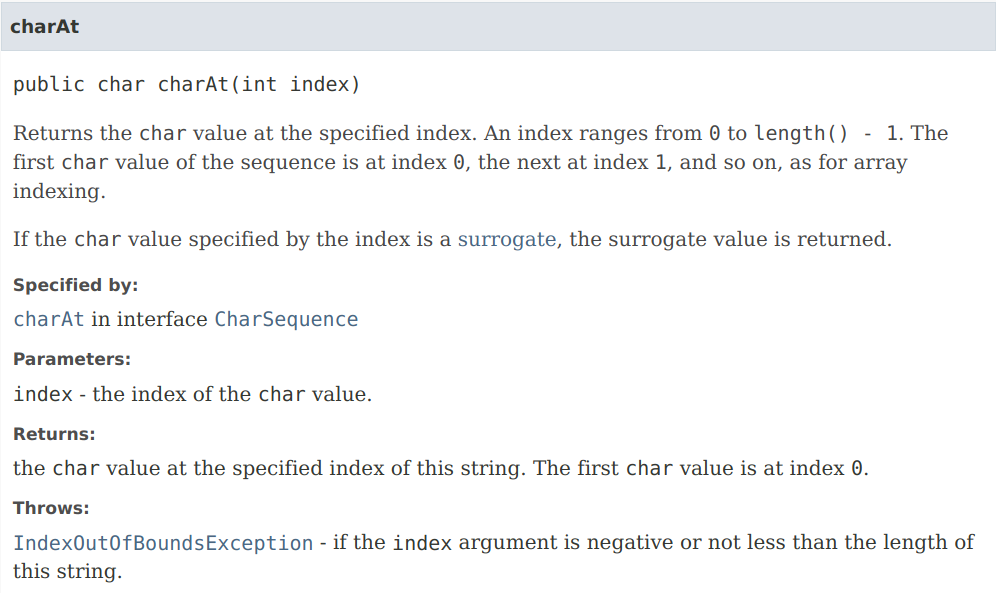
\includegraphics[width=0.75\textwidth]{figs/api-doc-charAt.png}
	\caption{API documentation for the \lstinline{charAt} method of the \lstinline{java.lang.String} class}
\end{figure}

Manual labelling is then required for the samples to identify the prevalence of different caveat types for the sentences. In  particular, the categories identified in \cite{zhou-directive} of \textit{not-null}, \textit{range limitation} and \textit{type restriction} are used as labels with the addition of \textit{ambiguous} to account for sentences that do not match any of the former classes. The \textit{not-null} category involves sentences that specify some parameter cannot be the \lstinline{null} value. The \textit{range limitation} category specifies some numerical limitation on a parameter such as a non-negative requirement. Finally, the \textit{type restriction} category indicates that a parameter must a particular class type or one of several types. The \textit{nullness allowed} category that was also identified is not considered because it only describes an acceptable condition for contracts, whereas the other categories describe the conditions that constitute an API misuse (or caveat). Overall, the results of this for the parameter sentences sample is shown in Table \ref{tab:caveat-param-stats}, while the results for exception level sentences is shown in Table \ref{tab:caveat-exception-stats}. We note that for \ref{tab:caveat-exception-stats}, the counts contribute add up to more than 356 because 6 of the labelled caveat samples fit both the \textit{not-null} category and the \textit{range limitation} category. 

\begin{table}[h]
	\centering
	\begin{tabular}{|l|cccc|}
		\hline
		& \multicolumn{4}{c|}{\textbf{Labels}} \\ \cline{2-5} 
		& \textbf{ambiguous} & \textbf{not-null} & \textbf{range limitation} & \textbf{type restriction} \\ \hline
		\textbf{Count} & 291 & 26 & 19 & 0 \\ \hline
	\end{tabular}
	\caption{Manually labelled results for classes of 336 randomly sampled parameter level caveat sentences.}
	\label{tab:caveat-param-stats}
\end{table}

\begin{table}[h]
	\centering
	\begin{tabular}{|l|cccc|}
		\hline
		& \multicolumn{4}{c|}{\textbf{Labels}} \\ \cline{2-5} 
		& \textbf{ambiguous} & \textbf{not-null} & \textbf{range limitation} & \textbf{type restriction} \\ \hline
		\textbf{Count} & 242 & 73 & 46 & 1 \\ \hline
	\end{tabular}
	\caption{Manually labelled results for classes of 356 randomly sampled exception level caveat sentences.}
	\label{tab:caveat-exception-stats}
\end{table}

From Table \ref{tab:caveat-param-stats}, it can be seen that approximately 8\% of unique parameter caveat sentences impose a \textit{not-null} constraint and approximately 6\% of the unique parameter caveat sentences impose a \textit{range limitation} constraint. Despite the small percentage of sentences in parameter sentences sample that fit these categories, it is important to note that they represent an important type of API caveats that can cause software failures from exceptions. Furthermore, these caveat types generally contain explicit constraint descriptions that have little dependencies on other API elements, making them simpler to parse and an adequate baseline for constructing caveat contracts. In contrast, the results from Table \ref{tab:caveat-exception-stats} show that a considerably larger subset of 20\% of unique exception caveat sentences specify a \textit{non-null} constraint. This is also observed for the \textit{range limitation} category with approximately 13\% of sentences labelled. \bigbreak

An analysis of other categories is also conducted to determine what other caveat contracts can be constructed. In particular, the categories identified in \cite{code-examples} are derived from API misuse patterns data-mined from code snippets on Stack Overflow, but can also be mapped into contracts. For example, \textit{missing control constructs} can be represented by a caveat contract that defines the control structure around some API call as a requirement. The same concept can also be applied to \textit{missing or incorrect order of API calls} and \textit{incorrect guard conditions}. For the subcategories of \textit{missing control constructs}, which include \textit{missing exception handling}, \textit{missing if checks} and \textit{missing finally}, we observe that they would all require explicit explanations for usage of these control structures. This is because usage of a control structure such as \lstinline{if} or \lstinline{finally} cannot be inferred without those stating those keywords. Furthermore, \textit{incorrect guard conditions} could be considered a superset of the constraints analysed previously in \cite{zhou-directive} for the Java API documentation, but sentences that do not fit a category identified by \cite{zhou-directive} could be expected to be rare occurrences. \bigbreak

I focus on \textit{missing control structures} and \textit{missing or incorrect order of API calls} as categories to analyse. Using a similar approach to before, the estimated sample size required is calculated with Equation \ref{sample} for sentences from the method/constructor description, parameter section or return value section, which are 321, 377, 336 and 353 respectively for unique sentence population sizes of 8,829, 22,465, 2704 and 4,426. The exception section sentences are not considered as they would all be categorised as descriptions of \textit{missing exception handling} or \textit{incorrect guard conditions}. This emphasises the fact that the exception sentences are an important subset of API caveats. The labelled results are shown in Table \ref{tab:caveat-sent-stats}. Note that \textit{Control} refers to \textit{missing control structures}, \textit{Temporal} refers to \textit{missing or incorrect order of API calls} and \textit{guard} refers to \textit{incorrect guard conditions}.\\

\begin{table}[h]
	\begin{tabular}{|cc|cccc|}
		\hline
		&  & \multicolumn{4}{c|}{\textbf{Labels}} \\ \cline{3-6} 
		&  & \textbf{Ambiguous} & \textbf{Control} & \textbf{Temporal} & \textbf{Guard} \\ \hline
		\multicolumn{1}{|c|}{\multirow{4}{*}{\textbf{Sentence Location}}} & \textbf{Constructor} & 264 & 21 & 6 & 32 \\ \cline{2-6} 
		\multicolumn{1}{|c|}{} & \textbf{Method} & 360 & 9 & 4 & 5 \\ \cline{2-6} 
		\multicolumn{1}{|c|}{} & \textbf{Parameter} & 257 & 2 & 2 & 75 \\ \cline{2-6} 
		\multicolumn{1}{|c|}{} & \textbf{Return} & 351 & 0 & 1 & 0 \\ \hline
	\end{tabular}
	\caption{Manually labelled categories for caveat sentences found in different locations of the Java 12 API documentation.}
	\label{tab:caveat-sent-stats}
\end{table}

The results in Table \ref{tab:caveat-sent-stats} show the size of \textit{Guard} caveat sentences is significantly larger in parameter sentences and the highest for constructor sentences. Meanwhile, method sentences have roughly equal caveat sentences belonging to the \textit{Control}, \textit{Temporal} or \textit{Guard} categories. Overall, this indicates that perhaps API documents rarely contain API methods that require specific call orders or additional control structures, and caveats related to some guard conditions are the most prevalent. This is an interesting result given that the most prevalent type of API misuse found by \cite{code-examples} for 66,897 Stack Overflow posts was related to \textit{missing control constructs}, followed by \textit{incorrect guard conditions} then \textit{missing or incorrect order of API calls}, which suggests that the Java 12 API documentation does not contain sufficient information for developers to handle API caveats involving control structures.

\subsection{API Contracts Construction}
\label{subsec:contract-construct}
Given the results found from statistical analysis in \ref{subsec:contract-caveat-statistics}, the next step is to collect a set of API caveat sentences and attempt to transform them into caveat contracts. As a baseline study, the API caveats contained within the \textit{not-null} and \textit{range limitation} categories were found to represent a sufficient proportion of exception caveat sentences (see Table \ref{tab:caveat-exception-stats}) and are therefore chosen. 
We note that this allows us to base our solution on the 64 heuristic rules and 29 regular expressions from \cite{zhou-directive} designed for parsing mainly \textit{not-null} and \textit{range limitation} constraints. For reference, the approach in \cite{zhou-directive} required intensive manual analysis to formulate the heuristics. Hence, extend upon the methods used with a key observation of English sentences and sentence normalisation techniques used by \cite{blasi2018translating} to propose a much simpler approach of extracting constraints and constructing caveat contracts in general. \bigbreak

To design a simpler method for parsing API caveats with a \textit{not-null} constraint, we observe that sentences must mention the term ``null'' to either specify if a \lstinline{null} value is allowed or not allowed in code. Furthermore, given the structural information of the Java 12 API documentation for parameter sentences and exception sentences, extracting additional information such as the subjects of the sentences is simple (as described in Section \ref{subsec:contract-caveat-statistics}). Therefore, dependency parsing POS tagging is not required. Another observation made based on the heuristics from \cite{zhou-directive} is the prevalence of the subject-verb-object (SVO) ordering for a given sentence \cite{dryer200581}. Specifically, English is known to follow SVO ordering despite other possible orderings such as subject-object-verb used in Japanese or subject-verb-object in Mandarin. This structure can be seen from rules 1 and 17 of Table \ref{tab:not-null-heuristic} and all shown in Table \ref{tab:range-limit-heuristic}. For rule 20, we observe the use of ``non-null` as a predicative adjective to the subject, which is the only \textit{non-null} heuristic formulated that has ``null'' appearing before the subject. The final observation for \textit{not-null} caveats is that whether some API method/constructor's parameter can be null is a boolean condition. In other words, this category of caveats represents the simplest form of a caveat contract as it only needs to specify whether a null value is accepted or not accepted. Given this information, a general approach to identify whether an API caveat is of the \textit{non-null} category is to filter out caveat sentences that do not contain the sub-string ``null''. Next, we assume that API documentation aims to be simplistic and mentions of nullness within certain sentences (i.e. parameter or exception sentences) can be regarded as a \textit{non-null} constraint. This is particularly true for the Java 12 API documentation as exception sentences (for example) describe the conditions required for the relevant exception to be thrown. Hence, any mention of ``null'' could be assumed to indicate a null value will result in an exception. We do note however that this assumption does not necessarily hold for other API documentation. \\

\begin{table}[h]
	\centering
	\begin{tabular}{|cc|}
		\hline
		Rule Number & Heuristic \\ \hline
		1 & [something] be/equals null \\
		17 & Value of [something] be/equals null \\
		20 & Non-null [something] \\ \hline
	\end{tabular}
	\caption{Example of 3 of 20 heuristic rules for nullness not allowed from \cite{zhou-directive}. Note that the complete list can be found in \ref{tab:not-null-heuristic} (Appendix).}
	\label{tab:not-null-heuristic}
\end{table}

\begin{table}[h]
	\centering
	\begin{tabular}{|cc|}
		\hline
		Rule Number & Heuristic \\ \hline
		1 & [something] >/</= [value] \\
		8 & [something] be {not} negative/positive/false/true \\
		20 & [something1] equals [something2] \\ \hline
	\end{tabular}
	\caption{Example of 3 of 23 heuristic rules for range limitations from \cite{zhou-directive}. Note that the complete list can be found in \ref{tab:range-limit-heuristic} (Appendix).}
	\label{tab:range-limit-heuristic}
\end{table}

An alternative approach for parsing the \textit{non-null} and \textit{range limitation} API caveats is to utilise sentence normalisation techniques used in \cite{zhou-directive} and \cite{blasi2018translating}. In particular, several regular expressions are identified by \citeauthor{zhou-directive} to perform substitutions within a sentence before dependency parsing. These expressions are used to detect cases such as the names of variables, classes, and mathematical expressions, which are then replaced with a predefined token to facilitate dependency parsing. This process is a form of \textit{sentence normalisation}. However, rather than using a dependency parser, we can simply use build heuristic rules based on the structure of SVO in English sentences. For example, a sentence in the exception section of the \lstinline{ArrayBlockingQueue} constructor for class \lstinline{java.util.concurrent.ArrayBlockingQueue<E>} says:

\begin{verbatim}
IllegalArgumentException - if capacity is less than c.size(), or less than 1
\end{verbatim}

If we ignore the exception, and focus on the description text after the hyphen as described in Section \ref{subsec:info-caveat-extract}, we obtain:

\begin{verbatim}
if capacity is less than c.size(), or less than 1
\end{verbatim}

From this, we can then apply sentence normalisation techniques previously used. The rules formulated for this project are shown in \ref{tab:normalisation-regex} and are based on those used by \cite{blasi2018translating}. These rules are used first in the normalisation process. For the given example, the first phase of normalisation results in:

\begin{verbatim}
if capacity is < c.size(), or < 1
\end{verbatim}

\begin{table}[h]
	\begin{tabular}{|l|l|}
		\hline
		\textbf{Regular Expression} & \textbf{Normalisation Form} \\ \hline
		(not? (less|shorter) than)|((greater|larger) than or equal to) & \textgreater{}= \\ \hline
		(not? (greater|larger|longer) than)|((less|shorter) than or equal to) & \textless{}= \\ \hline
		(less|shorter) than & \textless{} \\ \hline
		(greater|larger|longer) than & \textgreater{} \\ \hline
		((is|are)? not negative)|((be)? non-negative) & \textgreater{}=0 \\ \hline
		((is|are)? not positive)|((be)? non-positive) & \textless{}=0 \\ \hline
		(is|are)? negative & \textless{}0 \\ \hline
		(is|are)? positive & \textgreater{}0 \\ \hline
		not equal( to)? & != \\ \hline
		equal to & == \\ \hline
	\end{tabular}
	\caption{Regular expressions used to normalise mathematical phrases.}
	\label{tab:normalisation-regex}
\end{table}

The second phase of sentence normalisation involves the regular expressions shown in Table \ref{tab:zhou-regex} from \cite{zhou-directive}. This allows us to utilise the SVO structure of English to perform a greedy parsing approach. The result of this is:

\begin{verbatim}
if @PARAM1 is @EXPR1, or @EXPR2
\end{verbatim}

Here, ``@PARAM1'' represents ``capacity'', which is the first parameter of the method, and ``@EXPR1'' and ``@EXPR2'' represent the mathematical expressions within the sentence. Finally, we extract the constraints from the sentence by using exploiting the linear nature of the SVO structure that allows words of a sentence to be considered in sequence from left to right. We first we tokenise the sentence such that we have a list of tokens, then iterate over the list in a single pass. States are saved throughout the iteration process based on the token observed at each step of the iteration. These states contain information such as whether a negating word (e.g. ``not'', ``false'') or expression was encountered. A simplistic rule for the parsing is to then construct a caveat contract whenever an expression token is encountered. The last parameter observed so far is then used to complete this expression. For the given example, both ``@EXPR1'' and ``@EXPR2'' are therefore completed with ``@PARAM1'' to form the constraints $capacity<c.size()$ and $capacity<1$. We note that for the scope of this project, the rules used to construct these constraints are simplistic and only consider these mathematical constraints alongside logical ``or'' conditions as shown in the example above. However, this is sufficient to map API caveat sentences of the \textit{not null} and \textit{range limitation} categories.  Other constraint types such as temporal rules for API calls would require much more complex parsing techniques. \\

% Please add the following required packages to your document preamble:
% \usepackage{multirow}
\begin{table}[h]
	\centering
	\begin{tabular}{|l|l|l|}
		\hline
		\textbf{Type} & \textbf{Description} & \textbf{Regular Expression} \\ \hline
		\multirow{2}{*}{\shortstack[l]{Specific\\Values}} & 0.0, 0.1f, etc. & \textbackslash{}W(-)?{[}0-9{]}+(,{[}0-9{]}+)*((\textbackslash{}.{[}0-9{]}+)?{[}a-z{]}*)\textbackslash{}W \\ \cline{2-3} 
		& \begin{tabular}[c]{@{}l@{}}Member value of objects \\ e.g. Location.x\end{tabular} & \shortstack[l]{\textbackslash{}W(\textasciicircum{}(java\textbackslash{}.|javax\textbackslash{}.|org\textbackslash{}.))?\\({[}A-Za-z\_{]}+\textbackslash{}w+\textbackslash{}.)+{[}a-z\_{]}+{[}a-z0-9\_{]}*{[}\textasciicircum{}\textbackslash{}.A-Za-z0-9\_{]}} \\ \hline
		\multirow{4}{*}{\shortstack[l]{Class\\methods\\and\\static\\members}} & \begin{tabular}[c]{@{}l@{}}class methods,\\ e.g., ClassA.func(Param1)\end{tabular} & \shortstack[l]{\textbackslash{}W{[}A-Za-z\_{]}+{[}A-Za-z\_0-9{]}*(\textbackslash{}.{[}A-Za-z\_{]}+{[}A-Za-z\_0-9{]})*\\(\#{[}A-Za-z\_{]}+{[}A-Za-z\_0-9{]}*)?\([^()]*\)\textbackslash{}W} \\ \cline{2-3} 
		& \shortstack[l]{Static member,\\ e.g.  Desktop.Action\#OPEN} & \shortstack[l]{\textbackslash{}W({[}A-Za-z\_{]}+{[}A-Za-z\_0-9{]}*(\textbackslash{}.{[}A-Za-z\_{]}+\\{[}A-Za-z\_0-9{]})*)?(\#{[}A-Za-z\_{]}+{[}A-Za-z\_0-9{]}*){[}\textasciicircum{}A-Za-z0-9\_(){]}} \\ \cline{2-3} 
		& All upper case & \textbackslash{}W(\textbackslash{}w+\textbackslash{}.)*({[}A-Z{]}+\_)*{[}A-Z{]}+\textbackslash{}W \\ \cline{2-3} 
		& Class name & \shortstack[l]{\textbackslash{}W({[}A-Za-z\_{]}+\textbackslash{}w+\textbackslash{}.)*{[}A-Za-z\_{]}*{[}A-Z{]}+\\\textbackslash{}w+{[}\textasciicircum{}\textbackslash{}.A-Za-z0-9\_{]}} \\ \hline
		\multirow{11}{*}{Expressions} & A - B & \textbackslash{}W\textbackslash{}w+((\textbackslash{}s+-)|(-\textbackslash{}s+)|(\textbackslash{}s+-\textbackslash{}s+))\textbackslash{}w+\textbackslash{}W \\ \cline{2-3} 
		& A + B & \textbackslash{}W\textbackslash{}w+\textbackslash{}s*\textbackslash{}+\textbackslash{}s*\textbackslash{}w+\textbackslash{}W \\ \cline{2-3} 
		& A * B & \textbackslash{}W\textbackslash{}w+\textbackslash{}s*\textbackslash{}*\textbackslash{}s*\textbackslash{}w+\textbackslash{}W \\ \cline{2-3} 
		& A..B & \textbackslash{}W(?\textbackslash{}s*\textbackslash{}w+\textbackslash{}s*)?\textbackslash{}s*\textbackslash{}.\textbackslash{}s*\textbackslash{}.\textbackslash{}s*(?\textbackslash{}s*\textbackslash{}w+\textbackslash{}s*)?\textbackslash{}W \\ \cline{2-3} 
		& {[}A, B{]} & \textbackslash{}W[\textbackslash{}s*\textbackslash{}w+\textbackslash{}s*,\textbackslash{}s*\textbackslash{}w+\textbackslash{}s*]\textbackslash{}W \\ \cline{2-3} 
		& {[}A..B{]} & \textbackslash{}W[\textbackslash{}s*\textbackslash{}w+\textbackslash{}s*(\textbackslash{}.\textbackslash{}s*\textbackslash{}.\textbackslash{}s*)\textbackslash{}s*\textbackslash{}w+\textbackslash{}s*]\textbackslash{}W \\ \cline{2-3} 
		& A \textless{}\textbackslash{}\textless{}= B \textless{}\textbackslash{}\textless{}= C & \textbackslash{}W\textbackslash{}w+\textbackslash{}s*\&lt;=?\textbackslash{}s*\textbackslash{}w+\textbackslash{}s*\&lt;=?\textbackslash{}s*\textbackslash{}w+\textbackslash{}W \\ \cline{2-3} 
		& A \textgreater{}\textbackslash{}\textgreater{}= B \textgreater{}\textbackslash{}\textgreater{}= C & \textbackslash{}W\textbackslash{}w+\textbackslash{}s*\&gt;=?\textbackslash{}s*\textbackslash{}w+\textbackslash{}s*\&gt;=?\textbackslash{}s*\textbackslash{}w+\textbackslash{}W \\ \cline{2-3} 
		& From A to B & \textbackslash{}W(from\textbackslash{}s+)?\textbackslash{}w+\textbackslash{}s+to\textbackslash{}s+\textbackslash{}w+\textbackslash{}W \\ \cline{2-3} 
		& A != B & \textbackslash{}W\textbackslash{}w+\textbackslash{}s*!=\textbackslash{}s*\textbackslash{}w+\textbackslash{}W \\ \cline{2-3} 
		& Enumeration expression & \textbackslash{}W (\textbackslash{}s*\textbackslash{}w+\textbackslash{}s*)(,\textbackslash{}s*\textbackslash{}w+\textbackslash{}s*)+,?\textbackslash{}s*or\textbackslash{}s*\textbackslash{}w+\textbackslash{}W \\ \hline
	\end{tabular}
	\caption{The regular expressions identified in \textbackslash{}cite\{\} for sub-sentence substitutions and dependency parsing.}
	\label{tab:zhou-regex}
\end{table}

\subsection{Checker Programs}
\label{sec:code-checker}
The previous section described a solution for constructing caveat constructs and assumed that program analysis tools exist which can utilise these contracts. Fortunately, such tools exist and are contained within a field known as static code analysis \cite{1657940}. Static code analysis uses checker tools that can perform checks on other programs without executing them. A common data structure used by these tools is Abstract Syntax Trees (ASTs), which models the structure of source code as a tree. Syntactic details of the code are not represented which enable an analysis of code to be significantly simpler. Consider the following code for the Euclidean algorithm:

\begin{verbatim}
while b != 0
    if a > b
        a := a - b
    else
        b := b - a
return a
\end{verbatim}

The AST of the program is shown in \ref{fig:ast}. In particular, ASTs can be used to extract important information such as an API method call, what control structures (such as \lstinline{for} or \lstinline{if} blocks) they reside in, or what parameters are passed to the method. Given a caveat contract, we could traverse the AST of a program and identify any code expressions and statements that correspond to the relevant API element. Checking if a caveat contract is satisfied then requires one or more of the following processes: observing the surrounding API calls, identifying relevant expressions and statements, inspecting the various control flows of the program, evaluating expressions, and inspecting the API call parameters. \\
The IntelliJ platform was chosen for the development of a proof-of-concept plugin given that it was one of the three most popular Java IDEs (next to Netbeans and Eclipse) and provides a simple interface for accessing the AST of Java code. IntelliJ provides an interface known as the Program Structure Interface (PSI) that allows developers to interact with the AST of a program approaches to navigation of an AST, making the development of a plugin relatively simple.

\begin{figure}
	\label{fig:ast}
	\centering
	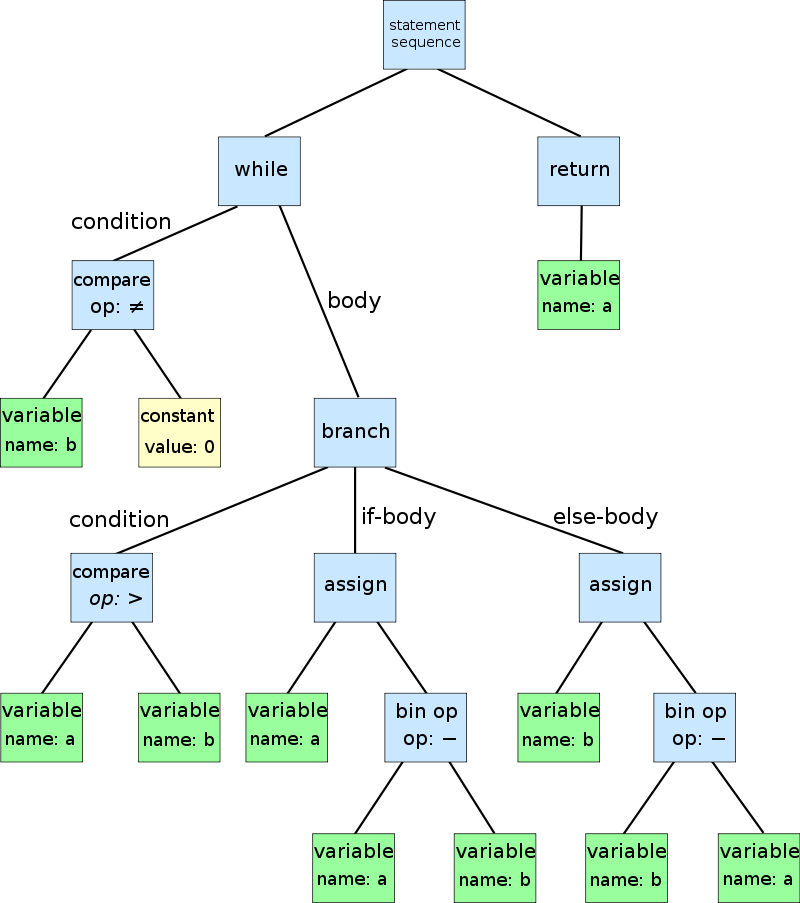
\includegraphics[width=0.75\textwidth]{figs/ast.png}
	\caption{Example of an AST for the Euclidean algorithm. Copied from \url{https://en.wikipedia.org/wiki/Abstract\_syntax\_tree}}
\end{figure}

\section{Implementation}
\label{sec:contract-implement}
Implementation of the caveat contract construction for the Java 12 API is completed using Python 3.6 and its standard libraries. The contracts generated are exported as a JSON array to be used in other applications (i.e. the plugin) and can be found in the project repository of the IntelliJ plugin (\url{./exception_range_rules_filtered.json}).

\subsection{Java API Caveat Contracts}
\label{subsec:contract-caveat-contracts}
The caveat sentences extracted from the previous chapter (Section \ref{subsec:info-caveat-extract}) was reused and loaded as a Pandas library\footnote{https://pandas.pydata.org/} \lstinline{DataFrame} object. The object consists of rows of individual caveats while the columns represent various information about a caveat such as the corresponding caveat sentence and which Java class it belonged to. This allowed filtering functions to be easily applied such that a subset of the caveats could be selected based on some condition. Constructing the caveat contracts involves following the approach described in \ref{subsec:contract-construct}. In particular, this involves defining the regular expressions from \ref{tab:zhou-regex} and \ref{tab:normalisation-regex} in Python's \lstinline{re} library syntax. A preprocessing step is then performed to reduce the set of caveat sentences that are clearly not \textit{not null} or \textit{range limitation} caveats. I create generalised regular expressions used to identify the caveat sentences that belong to these categories from the fact that sentences of the \textit{range limitation} category, for example, would likely contain soon mathematical logical operators such as ``<'' for less than/greater than. The regular expressions used can be found in Tables \ref{tab:except-null}, \ref{tab:param-null}, \ref{tab:except-range} and \ref{tab:param-range}. Applying these filters reduces the set of invalid caveat sentences and the amount of work required for manually labelling during evaluation.\bigbreak

\begin{table}[h]
	\centering
	\begin{tabular}{|l|}
		\hline
		\textbf{Regular Expression} \\ \hline
		null \\ \hline
	\end{tabular}
	\caption{Regular expressions for identifying exception sentences of the \textit{not-null} category.}
	\label{tab:except-null}
\end{table}

\begin{table}[h]
	\centering
	\begin{tabular}{|l|}
		\hline
		\textbf{Regular Expression} \\ \hline
		not( be)? null \\ \hline
		non-null \\ \hline
	\end{tabular}
	\caption{Regular expressions for identifying parameter sentences of the \textit{not-null} category.}
	\label{tab:param-null}
\end{table}

\begin{table}[h]
	\centering
	\begin{tabular}{|l|}
		\hline
		\textbf{Regular Expression} \\ \hline
		\textless{}|\textgreater{}|= \\ \hline
		equal|equal to|equivalent to|illegal value| is (nan|infinite|empty) \\ \hline
		\textbackslash{}b(less|smaller|greater|larger)\textbackslash{}b \\ \hline
		\textbackslash{}b(range|negative|positive|non-negative|non-positive)\textbackslash{}b \\ \hline
	\end{tabular}
	\caption{Regular expressions for identifying exception sentences of the \textit{range limitation} category}
	\label{tab:except-range}
\end{table}

\begin{table}[h]
	\centering
	\begin{tabular}{|l|}
		\hline
		\textbf{Regular Expression} \\ \hline
		\textless{}|\textgreater{}|= \\ \hline
		(less|smaller|greater|larger) than \\ \hline
		negative|positive|non-negative|non-positive \\ \hline
	\end{tabular}
	\caption{Regular expressions for identifying parameter sentences of the \textit{range limitation} category.}
	\label{tab:param-range}
\end{table}

Before the implementation of sentence parsing and contract construction, I random sampling to the sentences for evaluation purposes in later steps. The unique sentences from the \textit{not-null} exception and parameter sentences are identified, totalling 835 and 193 respectively. For the \textit{range limitation} category, the number of unique exception and parameter sentences is 193 and 149. I then randomly generate a sample of size 100 for each of these sets, which is an appropriate sample size given the small sets of unique sentences and overall simplicity. For the \textit{not-null} categories of exception and parameter sentences, the relevant parameter for the constraint (if any) was identified. As an example, for the sentence ``prefix - the prefix of the tag, may not be null'', \textit{prefix} would be marked as the constraint subject. Since the parameter sentences follow a template as described in \ref{subsec:contract-caveat-statistics}, we note that an algorithm to extract the relevant parameter is trivial whereas for an exception sentence like ``if the specified sorted set is null''\footnote{Taken from the constructor of \lstinline{java.util.TreeSet<E>}}, parsing is harder given that the name of the relevant parameter (``s'' in this case) is not used. \bigbreak

Labelling of the \textit{range limitation} sentences was completed by expressing constraints as mathematical expressions. An example of this is with the sentence ``IllegalArgumentException - if iv is null or (iv.length - offset < 2 * (wordSize / 8))''\footnote{ Taken from the \lstinline{RC5ParameterSpec} constructor of the \lstinline{javax.crypto.spec.RC5ParameterSpec} class}, the constraint of the sentence would be identified as $iv.length-offset<2*(wordSize/8)$. After manual labelling, 90\% of the 100 random parameter sentences filtered for \textit{not-null} were found to actually describe a \textit{not-null} constraint. For the exception level sentences, 87\% were found to describe a \textit{not-null} constraint. For the \textit{range-limitation} samples, 49\% and 72\% of the parameter and exception sentences were found to express a \textit{range limitation} constraint, respectively. These results reveal that using basic sub-string searches is viable for identifying \textit{not-null} constraints, but more complex approaches are required for identifying (and extracting) \textit{range limitation} caveats. \bigbreak

For implementing the sentence parsing, we only focus on the exception sentences as a baseline. The sentence normalisation approach is implemented as described in \ref{subsec:contract-construct}, with regular expression from Tables \ref{tab:zhou-regex} and \ref{tab:normalisation-regex} used to perform substitutions with labelled words. The exception sentences are then tokenised by white-space characters and a simple \lstinline{for} loop is used to iterate through the tokens of each sentence. Constraints are then extracted throughout the iteration process when incomplete expression tokens are observed as described previously. Caveat contracts are then constructed and represented as individual objects that contain the associated class, and API element name, alongside the parameter name, constraint operator (such as the ``<'' operator to represent less than) and comparison value. This process results in 4,694 unique caveat contracts. We note that other representations might be required for other caveat categories, but this is sufficient for \textit{not null} and \textit{range limitation} caveats and for use by a checker program. \bigbreak

Manually comparing the caveat contracts constructed and the mathematical expressions from earlier, 41 of the 72 API caveat sentences that contain a range limitation constraint were correctly extracted. Furthermore, the approach was able to extract partially correct constraints for 13 other caveat sentences (where we define partial as some constraints that would also cause an exception was identified). Hence, 54 of the caveat sentences had caveat contracts that could be applied to static code analysis. We note that the approach proposed also collects caveats of the \textit{not null} category by simply using an equality operator (``='' or ``!=''). Due to this fact, I only focus on caveat constructs using this method and the alternative method proposed using basic keyword searching is not included in Section \ref{subsec:contract-plugin}. \\
Overall, the results found are represented in terms of a confusion matrix in \ref{tab:conf-mat} to allow computation of accuracy, precision, recall, and F-measure scores. It can be seen that the true positive (TP) is 54, true negative (TN) is 25, false positive (FN) is 2, and the false negative is 19. Using the equations \ref{accuracy}, \ref{recall}, \ref{precision} and \ref{f-measure}, the accuracy is 0.77, recall is 0.73, precision is 0.96 and F1 score is 0.83. These results suggest that applying a simplistic sentence normalisation is a viable approach for extracting constraints from sentences that describe exceptions thrown under certain conditions. 

\begin{table}[h]
	\centering
	\begin{tabular}{l|l|l|}
		\cline{2-3}
		& \textbf{Predicted Non-constraint} & \textbf{Predicted Constraint} \\ \hline
		\multicolumn{1}{|l|}{\textbf{Actual Non-constraint}} & 25 & 2 \\ \hline
		\multicolumn{1}{|l|}{\textbf{Actual Constraint}} & 19 & 54 \\ \hline
	\end{tabular}
	\caption{Confusion matrix for the sentence normalisation approach proposed.}
	\label{tab:conf-mat}
\end{table}

\begin{equation}
\label{accuracy}
\text{accuracy} = \frac{TP + TN}{TP + TN + FP + FN}
\end{equation}

\begin{equation}
\label{recall}
\text{recall}=\frac{TP}{TP + FN}
\end{equation}

\begin{equation}
\label{precision}
\text{precision}=\frac{TP}{TP + FP}
\end{equation}

\begin{equation}
\label{f-measure}
\text{F1}=\frac{2\cdot recall\cdot precision}{recall + precision}
\end{equation}

\subsection{IntelliJ Plugin with Static Code Analysis}
\label{subsec:contract-plugin}
IntelliJ's PSI provides the \lstinline{AbstractBaseJavaLocalInspectionTool} class that can be extended for creating plugins involving static code analysis. This was used to define a \textit{visitor} that would traverse the AST of a program periodically. In addition to this, classes were defined for the concepts of an API method, API class, caveat, and for storing a collection of all caveat contracts loaded from \ref{subsec:contract-caveat-contracts}. Java's \lstinline{HashMap} was used as the underlying data structure for storing the caveat contracts. This tree-like structure allowed searching for the contracts of an arbitrary method to consist of two simple steps: obtaining the methods attached to a certain class (via the full class name as a hash), finding the correct method by searching through the associated list of methods. It is noted that further optimisations could be used in the future to quicken the retrieval of contracts for a given API method such as using the hash of the method signature to map directly to its caveat contracts. However, a simple design was chosen given that the plugin was a proof-of-concept application. Overall, the code analysis process involved implementing the visit function for the visitor such that each expression call in the program would be analysed. Specifically, the full class name, method name and argument types would be identified. The caveat contracts associated to the API call would then be retrieved. Each caveat contract would then be invoked and checked given the argument values provided to the API call. For the \textit{not-null} constraints, this check simply required comparing the argument values to \lstinline{null}. For the \textit{range limitation} constraints, the logical operators ($<$, $\leq$, etc.) were also included alongside the comparing value in the contracts constructed from \ref{subsec:contract-caveat-contracts}. This meant that an SMT solver was not required and we could simply applying the range constraints in Java code, though an SMT solver could be used in future for more complex constraints. We also note here that as baseline checker program, we only analyse argument values passed directly to an API call. Furthermore, the caveat categories of interest for this thesis are \textit{not-null} and \textit{range limitation}, which do not require further analysis of a program's AST even though more complex analysis can be conducted (such as evaluating expressions/variables that are passed as arguments to an API call). IntelliJ's PSI then provides the functionality to register a problem that will be displayed within the code editor of the IDE. Each caveat contract that was found to be violated would then result in a problem to be registered for the associated API call.

\section{Results}
\label{sec:contract-results}
From the construction of caveat contracts for the Java 12 API documentation, and from the checker plugin implemented for IntelliJ, a proof-of-concept for applying natural language to source code was completed. To showcase an example of the plugin's functionalities, \ref{fig:plugin-inspection-off} illustrates several constraint-violating API calls for Java 12 API elements in IntelliJ. Using the plugin, the result is each constraint-violation is highlighted in IntelliJ with red squiggly lines as shown in \ref{fig:plugin-inspection-on}. Hovering the cursor over any of these highlighted problems will bring show a pop-up that provides more detailed information about the caveat contract violation. An example of this is shown in \ref{fig:plugin-problem}. In these examples, IntelliJ version 2018.2.4 (community edition) was used.

\begin{figure}[h]
	\label{fig:plugin-inspection-off}
	\centering
	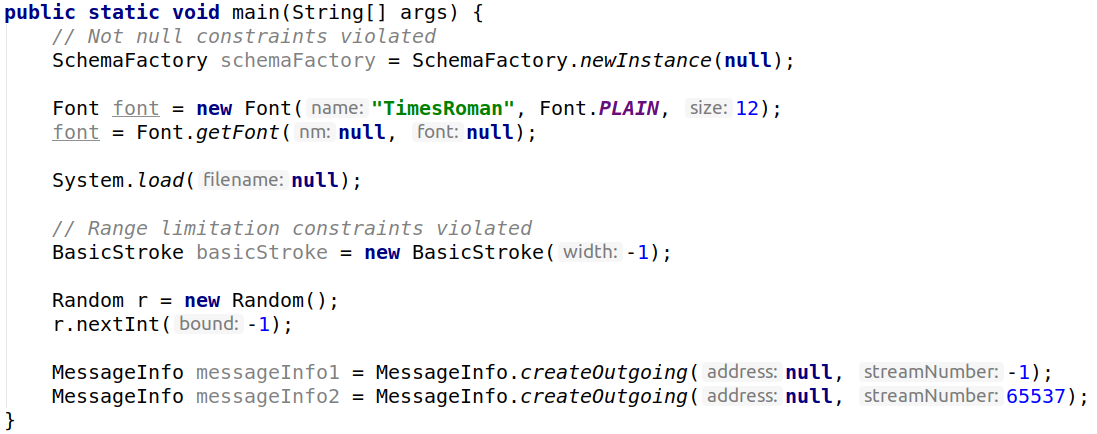
\includegraphics[width=0.85\textwidth]{figs/plugin-inspection-off.png}
	\caption{Example of IntelliJ's (lack of) problem highlights for obvious constraint violations.}
\end{figure}

\begin{figure}[h]
	\label{fig:plugin-inspection-on}
	\centering
	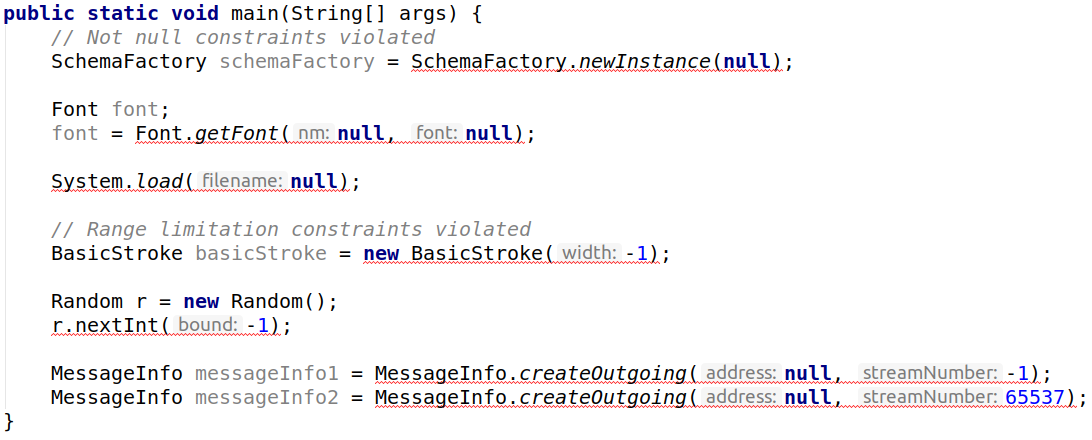
\includegraphics[width=0.85\textwidth]{figs/plugin-inspection-on.png}
	\caption{Example of how the developed plugin handles API caveat contract violations.}
\end{figure}

\begin{figure}[h]
	\label{fig:plugin-problem}
	\centering
	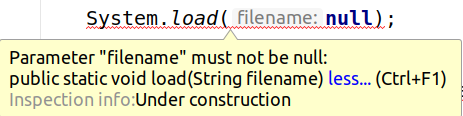
\includegraphics[width=0.3\textwidth]{figs/plugin-problem.png}
	\caption{Example of displayed problem message for an API caveat contract violation using the plugin.}
\end{figure}

It is noted that IntelliJ does implement its own version of contracts that require annotations following a specific syntax within the IDE. However, these contracts must be manually implemented for each method and were found to be mostly inconsistent. An example of this inconsistency is shown in \ref{fig:intellij-inspection-on} and \ref{fig:intellij-inspection-off}. In \ref{fig:intellij-inspection-on}, a \textit{not-null} constraint is violated for the \lstinline{isAfter} API call and correctly highlighted by IntelliJ's contracts. In \ref{fig:intellij-inspection-off}, another \textit{not-null} constraint is violated for the \lstinline{add} method of a \lstinline{PriorityQueue} object, which throws a \lstinline{NullPointerException} if executed. Hence, it can be seen that the code contracts implementation has two major drawbacks: it requires manual implementation of IntelliJ contracts for each method, and it is inconsistent (potentially as a result of the first problem). The plugin implemented is able to solve the first problem by automating the process of mapping sentences from the Java 12 API documentation to custom caveat contracts. Furthermore, it is able to solve the second problem with manual intervention as constraints for each individual API element are extracted and parsed into caveat contracts.

\begin{figure}[h]
	\label{fig:intellij-inspection-on}
	\centering
	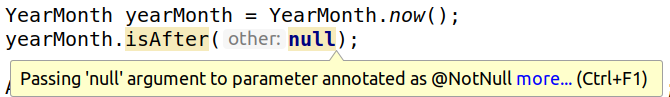
\includegraphics[width=0.5\textwidth]{figs/intellij-inspection-on.png}
	\caption{Example of IntelliJ's contracts.}
\end{figure}

Overall, the plugin in its current iteration is able to highlight the explicit contract violations from the Java 12 API documentation related to \textit{not-null} or \textit{range limitation} constraints. It is clear that with the addition of other categories of API caveats mapped to contracts, the plugin could be used to highlight many errors and problems for developers in real-time, which could minimise API misuse and help developers learn correct usage of an API. In terms of constructing caveat contracts, further research could yield methods that both improve the precision and recall of constraints extraction. It could also be used to bridge the gap between developers of an API and users of the given APIs such that API misuses can be minimised. In terms of static code analysis, the plugin shows that natural language can be applied to source code to improve understanding of an API, avoid API misuses and potentially increase efficiency of learning/development for programmers.

\begin{figure}[h]
	\label{fig:intellij-inspection-off}
	\centering
	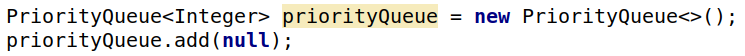
\includegraphics[width=0.5\textwidth]{figs/intellij-inspection-off.png}
	\caption{Example of IntelliJ's contract inconsistency.}
\end{figure}

\section{Summary}
\label{sec:contract-summary}
This chapter focused on the concept of code contracts and associated it to API caveats. The idea of transforming API caveats to contracts was presented and implemented for a subset of API caveats that were related to \textit{not-null} and \textit{range limitation} constraints. A statistical analysis was also performed to determine the prevalence of these categories of caveats in the Java 12 API documentation. It was found that 20\% of unique API caveat sentences appearing in the exception sections of the documentation imposed a \textit{not-null} constraint. For the \textit{range limitation} category, 13\% of unique API caveat sentences were found to describe a constraint involving range. These categories were chosen for investigation and implementation of code contracts as they were explicit constraints that would result in an exception and could be considered the baseline API caveats for mapping natural language to code contracts. Furthermore, a sentence normalisation algorithm was proposed for extracting the range constraints from sentences and used to construct 4,694 unique contracts. Design and implementation of a proof-of-concept IntelliJ plugin that acted as checker for the the caveat contracts was also presented. The potential of this approach for linking natural language to source code was also discussed. In particular, the plugin showcases that API misuses could be detected in real-time, improve understanding of APIs and direct developers to correct usage of an API.\\
In Chapter \ref{cha:conc}, the findings of this thesis are summarised and ideas for future work are presented. Lastly, some final remarks about the research focus of this thesis are expressed.

\chapter{Conclusion}
\label{cha:conc}
In this chapter, I summarise the topic of investigation, the main challenges identified in Chapter \ref{cha:intro} and how they relate to the main contributions of this thesis and make suggestions for future work. \bigbreak

Section \ref{sec:summary} provides an overview of this thesis in terms of topic, challenges, contributions and findings.\bigbreak

Section \ref{sec:future} describes some future work ideas relevant to API caveats and constructing API caveat contracts.\bigbreak 

\section{Summary}
\label{sec:summary}
This thesis presents the approach of using sentence embedding techniques to link Java 12 API caveats to community text from GitHub. Besides this, the complete process of constructing caveat contracts from API documentation (and its applications) is explored. Chapter \ref{cha:intro} introduced the concept of API caveats. A realistic scenario was provided to describe the motivation for linking API caveats to code, and the main challenges of this thesis were identified. Chapter \ref{cha:background} presented related work that defines the key concepts of this thesis: API caveats, using NLP techniques to augment API caveats with code examples, and the applications of static code analysis with API documentation. In Chapter \ref{cha:infoRetrieval}, the process of extracting the documentation and caveats from the Java 12 API was described in detail alongside the extraction process of GitHub community text data. The construction of multiple information retrieval systems based on TF-IDF, word2vec, BM25 was also documented. The negative results of this approach were discussed and used to introduce an alternative method applied in Chapter \ref{cha:codeAnalysis}. Chapter \ref{cha:codeAnalysis} presented the idea of caveat contracts and the transformation of API caveats to form caveat contracts. The design and implementation of a checker program that could utilise the caveat contracts was presented.\bigbreak

The main challenges of this thesis (Chapter \ref{cha:intro}) revolve around how API caveats can be linked to code. The challenges consist of effective sentence embedding and matching, sentence parsing techniques to extract constraints and the use of static code analysis with caveat contracts. In Chapter \ref{cha:infoRetrieval}, I tackled the problem of sentence embedding and matching by extending the work of \cite{jiamou} with additional information retrieval system models. Specifically, I constructed systems based on TF-IDF, word2vec, BM25 and word2vec + BM25 to investigate the differences of embedding models and how this approach performed with GitHub data. I attempted to match 73,831 API caveat sentences against 629,933 GitHub comment sentences using the models mentioned and performed statistical sampling with manual labelling to determine the performance of these information retrieval systems. However, a significant lexical gap was observed given that only 1\% of query results were found relevant to their API caveat queries. The negative result of this reveals that linkage via sentence embeddings cannot be performed in the presence of large lexical gaps. \bigbreak

In Chapter \ref{cha:codeAnalysis}, I tackled the challenges of sentence parsing for constraints extraction by utilising and combining ideas from \cite{zhou-directive} and \cite{blasi2018translating} to propose a sentence normalisation approach. I conducted a statistical analysis of the Java 12 API documentation for constraints recognised in \cite{zhou-directive} as \textit{not-null} and \textit{range limitation} constraints to showcase their prevalence in the Java API documentation. I found that 20\% of unique caveat sentences from exception sections of the documentation specify a \textit{non-null} constraint, while approximately 13\% of these sentences specify a \textit{range limitation} constraint. I then approached the challenges of static code analysis by developing a proof-of-concept checker and showing how it could detect caveat contract violations. This process involved the construction of 4,694 unique caveat contracts and an IntelliJ plugin that analysed code in real-time. 

\section{Future Work}
\label{sec:future}

\noindent
\textbf{Extending caveat contracts to include other caveat categories.} Other interesting caveat types mentioned in Chapter \ref{cha:intro} should also be considered for caveat contracts. These require much more complex parsing techniques. In addition, other methods to resolve dependencies of API caveats should be investigated. For example, the ``add'' method of ``ArrayList'' in Java specifies ``IndexOutOfBoundsException - if the index is out of range (index < 0 || index > size())''. Identifying that ``size()'' refers to the \lstinline{size} method of \lstinline{ArrayList} is a complex problem given that cross-element and cross-class dependencies exist.\\

\noindent
\textbf{Detecting bugs in existing software and performing more complex static code analysis.} The automatic detection of bugs remains a challenging problem. Two notable works that the methods proposed in this thesis can be combined with is \cite{code-examples}, which uses API call sequences to detect bugs, and \cite{mutation-analysis}, which uses mutation analysis to detect bugs. In \cite{code-examples}, the Boa programming language is used as an interface to a large number GitHub repositories and associated ASTs, used to data-mine correct usage patterns of APIs. Caveat contracts could be applied to this to detect API misuse in free, open-source software. They could also be integrated into development pipelines as automated tests that are performed before code is uploaded to GitHub. Besides this, methods to effectively present these errors and suggest fixes to developers still require further research as this thesis only identifies misuse after it has occurred. More complex static analysis for special API caveats, such as those that deal with the temporal order of API calls, is another topic for investigation. For \cite{mutation-analysis}, I suggest the topic of mutating caveat contracts to create correct code usage patterns. Specifically, this could be used to generate test suites that add an extra layer of code validation and overall development efficiency.\\

\noindent
\textbf{Testing other APIs, programming languages and natural languages.} Evaluating the practicality of caveat contracts and their construction for other APIs is a useful topic that should be investigated. This is because differing results can be expected for even minor differences in languages/APIs. Furthermore, the different syntactic styles used by developers for documentation presents a challenge for sentence parsing. Methods to construct caveat contracts for other languages (like Mandarin) would be valuable.

%%%%%%%%%%%%%%%%%%%%%%%%%%%%%%%%%%%%%%%%%%%%%%%%%%%%%%%%%%%%%%%%%%%%%%
% Here begins the end matter

% \appendix
\section{Heuristic Rules from \cite{zhou-directive}}
\subsection{Not-null Heuristics}
\label{app:not-null}
\begin{table}[]
	\begin{tabular}{|c|c|}
		\hline
		\textbf{Rule} & \textbf{Nullness Not Allowed Heuristics (@exception or @throws)} \\ \hline
		1 & [something] be/equals null \\ \hline
		2 & [something] be equal/equivalent to null \\ \hline
		3 & [something1] or [something2] be/equals null \\ \hline
		4 & [something1] or [something2] be equal/equivalent to null \\ \hline
		5 & [something] parameter be null \\ \hline
		6 & The specified [something] be null \\ \hline
		7 & Any/none of [something] be null \\ \hline
		8 & Either/neither/any/all/both/none parameter(s) be/equals null \\ \hline
		9 & Either/neither/any/all/both/none parameter(s) be equal/equivalent null \\ \hline
		10 & Either/neither [something1] or/nor [something2] be/equals null \\ \hline
		11 & Both [something1] and [something2] be null \\ \hline
		12 & The [type] be null \\ \hline
		13 & [parameter phrase] be/equals null \\ \hline
		14 & [parameter phrase] be equal/equivalent null \\ \hline
		15 & [something]’s value be/equals null \\ \hline
		16 & [something]’s value be equal/equivalent null \\ \hline
		17 & Value of [something] be/equals null \\ \hline
		18 & Value of [something] be equal/equivalent null \\ \hline
	\end{tabular}
	\caption{Complete list of heuristic rules for exception nullness not allowed.}
	\label{tab:complete-not-null-heuristic-except}
\end{table}

\begin{table}[]
	\begin{tabular}{|c|c|}
		\hline
		\textbf{Rule} & \textbf{Nullness Not Allowed Heuristics (@param)} \\ \hline
		19 & [something] can not be null \\ \hline
		20 & Non-null [something] \\ \hline
	\end{tabular}
	\caption{Complete list of heuristic rules for parameter nullness not allowed.}
	\label{tab:complete-not-null-heuristic-param}
\end{table}

\subsection{Range Limitation Heuristics}
\label{app:range-limit}
\begin{table}[]
	\begin{tabular}{|c|l|}
		\hline
		\textbf{Rule} & \textbf{Range Limitation Heuristic (@exception or @throws)} \\ \hline
		1 & [something] >/</= [value] \\ \hline
		2 & [something] be \{not\} less/greater/larger/equal/equivalent than/to [value] \\ \hline
		3 & [something] equals [value] \\ \hline
		4 & \makecell{[something1] or/and [something2] be \{not\} \\ less/greater/larger/equal/equivalent than/to [value]} \\ \hline
		5 & \makecell{Computing [expression] be {not} \\ less/greater/larger/equal/equivalent than/to [value]} \\ \hline
		6 & \makecell{Computing either [expression1] or [expression2] be \\ \{not\} less/greater/larger/equal/equivalent than [value]} \\ \hline
		7 & \makecell{Product/sum of [something1] and [something2] be \\ {not} less/greater/larger/equal/equivalent than/to [value]} \\ \hline
		8 & [something] be {not} negative/positive/false/true \\ \hline
		9 & [something1] or/and [something2] be {not} negative/positive/false/true \\ \hline
		10 & [something1] and [something2] be {not} the same \\ \hline
		11 & [something1] equals [something2] \\ \hline
		12 & [something] be {not} in/out of/outside of range [range value] \\ \hline
		13 & [something] be {not} in/out of bounds \\ \hline
		14 & [something] be {not} [value] \\ \hline
		15 & [range expression] (only the expression,like ) \\ \hline
		16 & [something] be {not} between [value1] and [value2] \\ \hline
		17 & [something] be {not} [value set] \\ \hline
		18 & [something] be {not} one of [value set] \\ \hline
		19 & [something] be {not} one of following: [value set] \\ \hline
		20 & [something] be {not} one of supported data, which are [value set] \\ \hline
	\end{tabular}
	\caption{Complete list of heuristic rules for exception range limitations.}
	\label{tab:complete-heuristics-range-limit-except}
\end{table}

\begin{table}[]
	\begin{tabular}{|c|c|}
		\hline
		\textbf{Rule} & \textbf{Range Limitation Heuristic (@param)} \\ \hline
		21 & [something] can/must {not} be negative/positive/non-negative/non-positive \\ \hline
		22 & [something] must be greater/less/larger than [value] \\ \hline
		23 & [something] be greater/less/larger than [value] \\ \hline
	\end{tabular}
	\caption{Complete list of heuristic rules for parameter range limitations.}
	\label{tab:complete-heuristics-range-limit-param}
\end{table}

\backmatter

\bibliographystyle{anuthesis}
\bibliography{thesis}

\printindex

\end{document}
